\chapter{Representative numerical simulations II}
\label{numerical-simulations-2}

\todo{\begin{itemize}
  \item Work on this after, and in tandem with, Chapter 4
  \item Weave around the monolithic implementation details and refer
    COMSOL's documentation to see how it goes about doing things?
    (Cite back to the fact that monolithic is stable.)
  \item Figure out the feasibility of: elastica, visco-poro-elasticity
    friction-coeff. variation or drop the entire section.
  \item Generate pristine plots for the flow field calculations and
    write up elaborate descriptions of the problems, citing back to
    the boundary conditions/saturation constraint of the previous
    chapter. Justify 2D.
  \item Bring in a few experimental figures and point out what we're
    looking for in terms of biphasic response.
  \item Go through cool/realistic calculations and replot a few from
    useful cases. Look at the new proposal to see what is sellable.
  \item Cite work from cancer to motivate the example. Generate many
    plots of the different fields and describe in great detail the toy
    problem citing back to Onsager reciprocity.
\end{itemize}}

\section{The coupled solution scheme}
\label{coupled-solution-scheme-2}

The second set of numerical simulations reside here.

\section{Material modelling}
\label{material-modelling}

\subsection{Elastica-based strain energy}
\label{elastica-stain-energy}

\subsection{Non-linear viscoelasticity}
\label{non-linear-viscoelasticity}

\begin{figure}[!hpt]
\centering
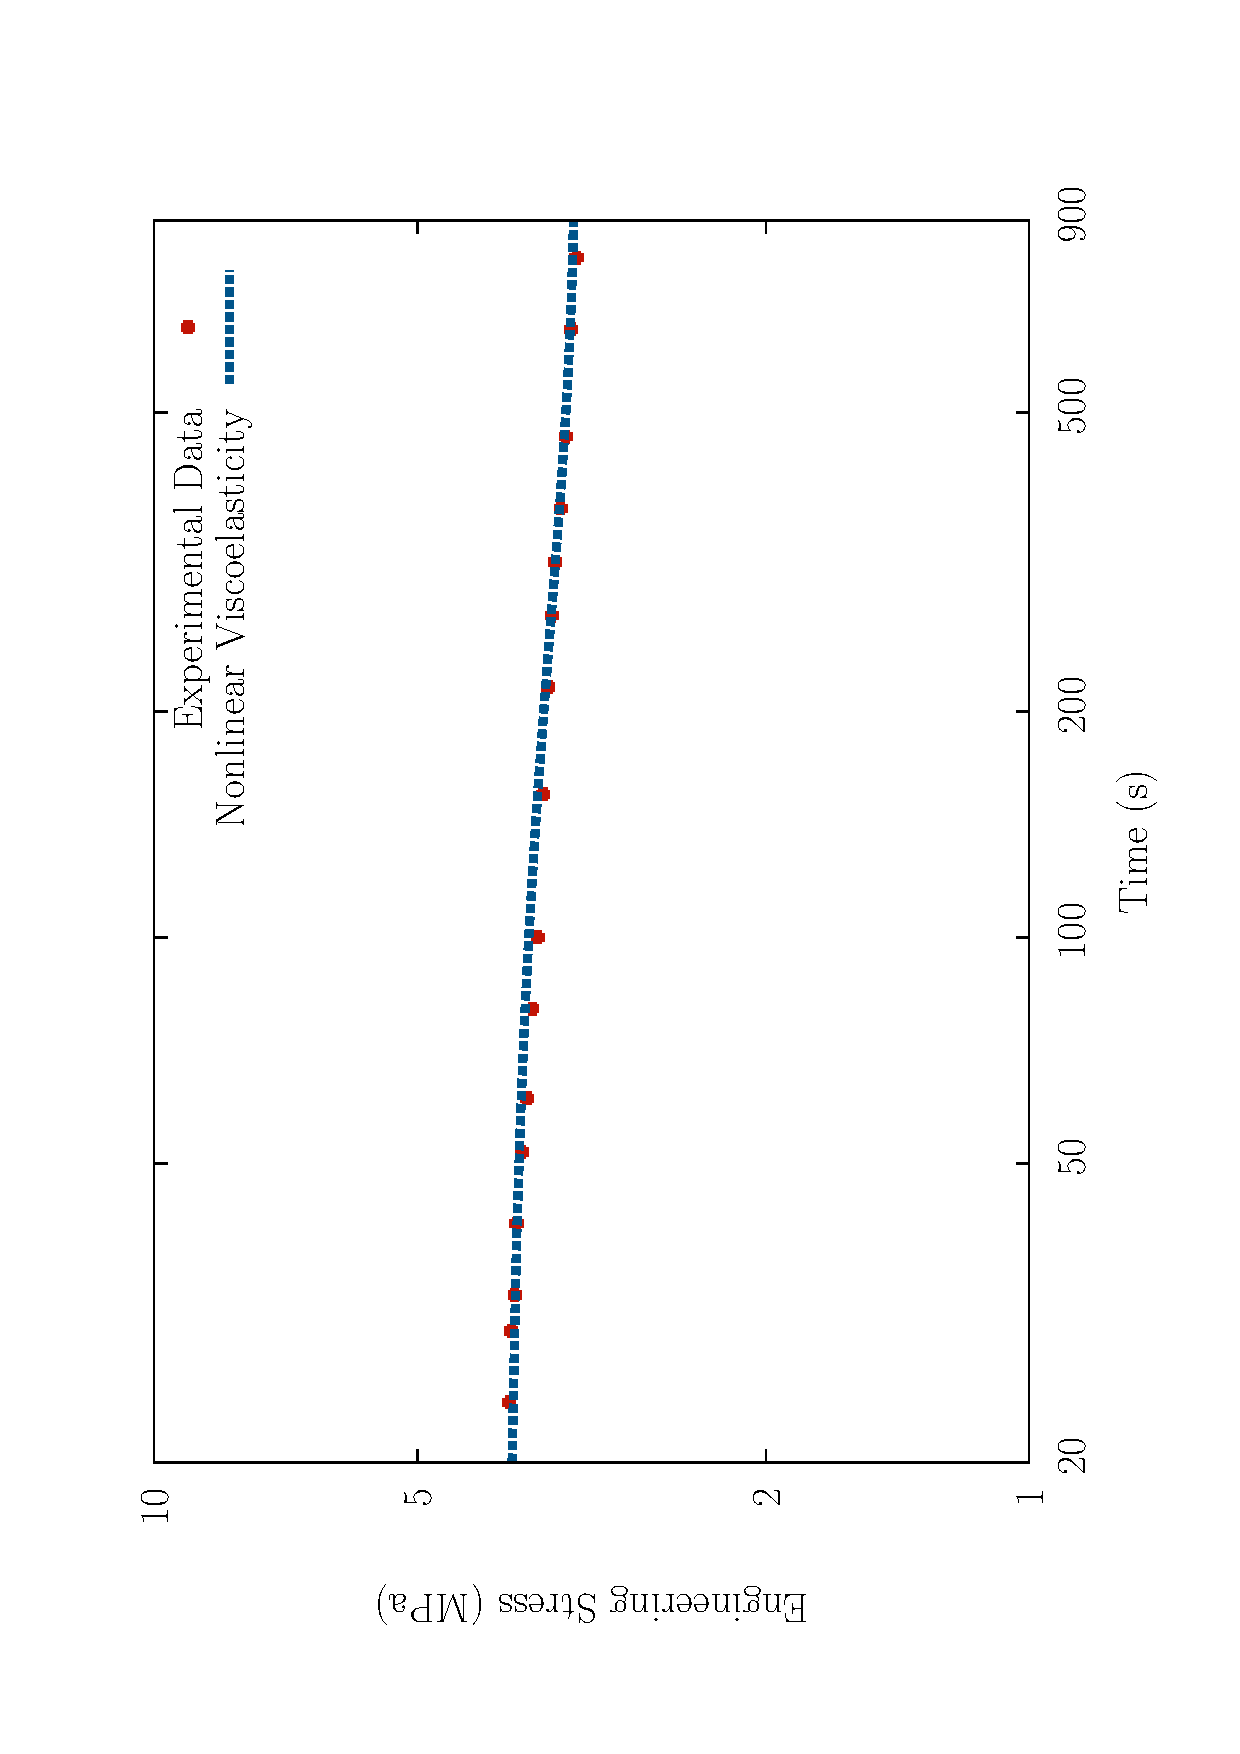
\includegraphics[width=0.6\textwidth,angle=270]{images/examples/eulerian/viscoelasticity/provenzano-data-comparison}
\caption{The non-linear time constants fit to experiment.} 
\label{provenzano-data-fit}
\end{figure}

\begin{figure}[!hpt]
\centering
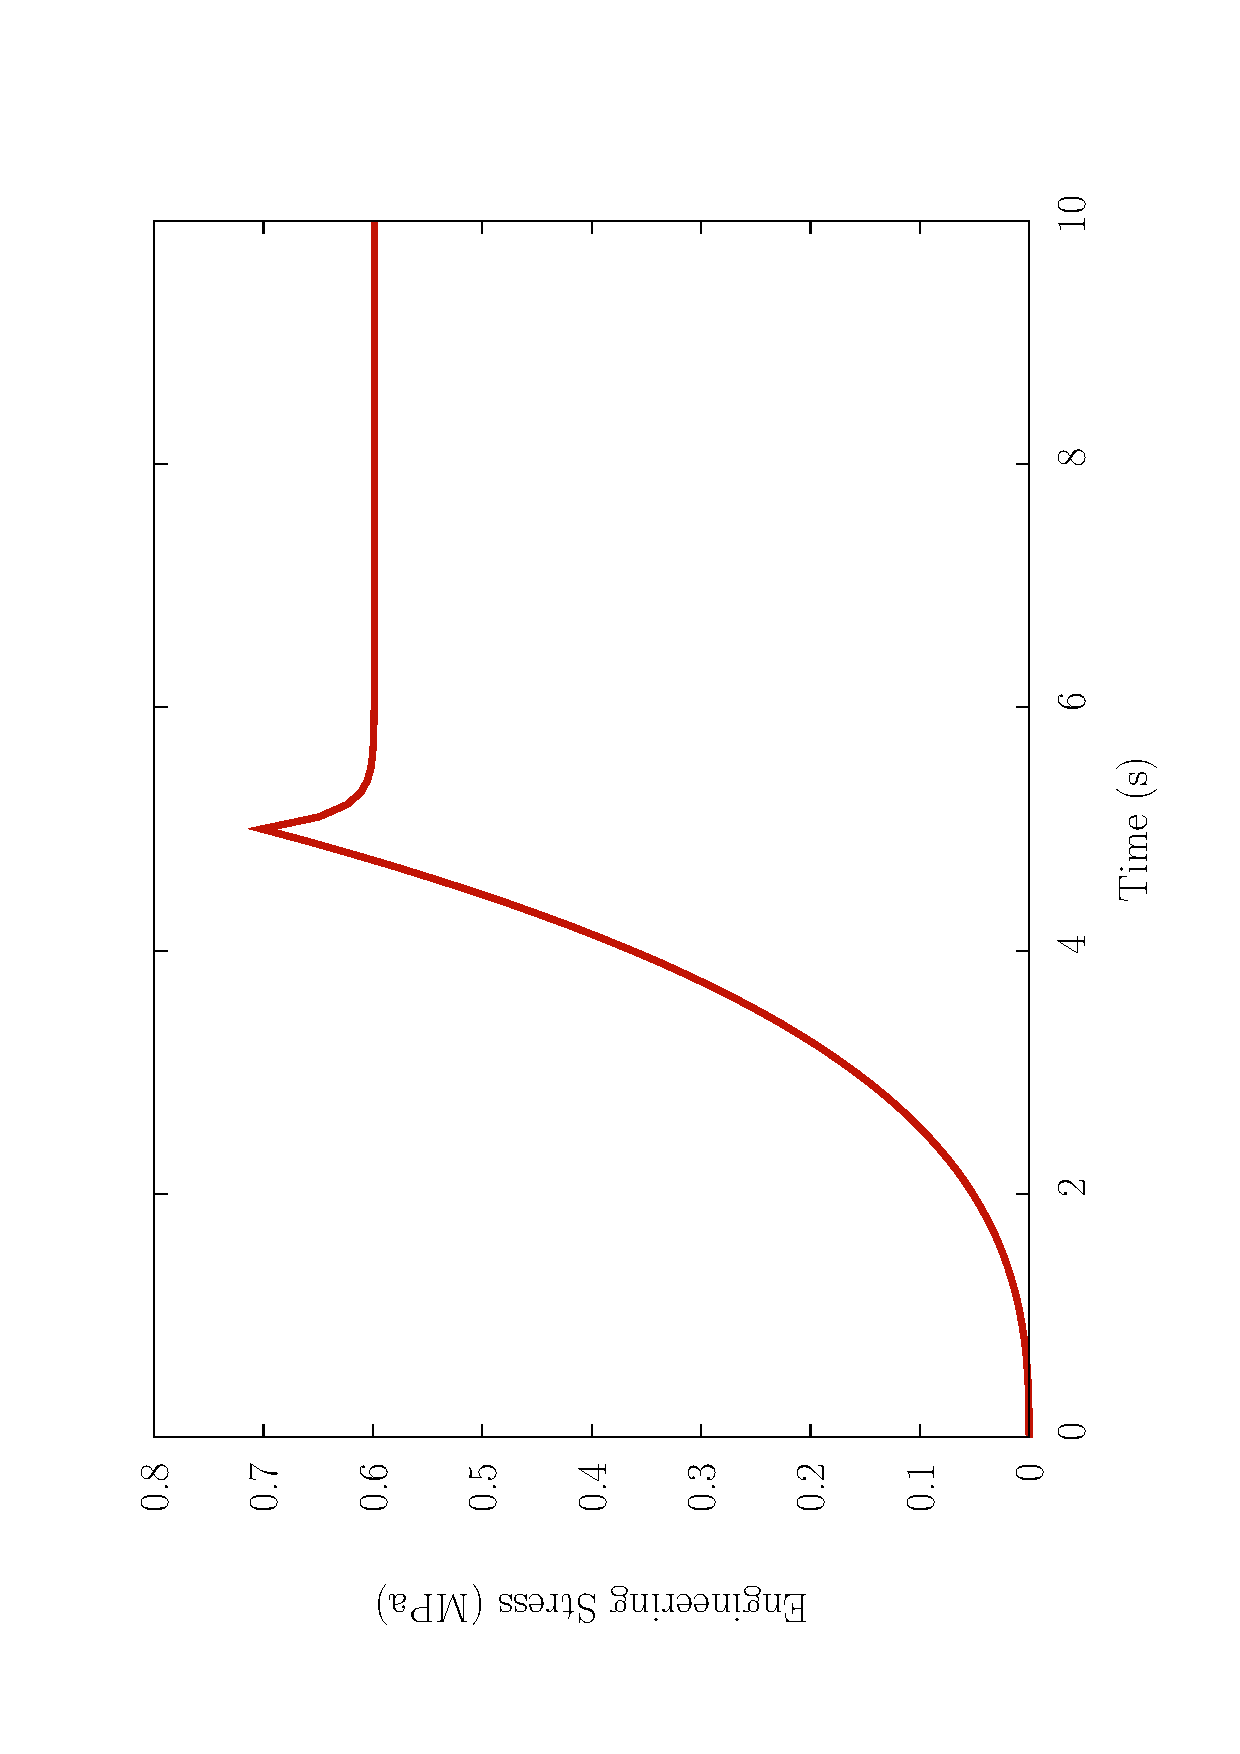
\includegraphics[width=0.6\textwidth,angle=270]{images/examples/eulerian/viscoelasticity/nonlinear-viscoelasticity-stress-relaxation}
\caption{Stress relaxation under nonlinear viscoelasticity.}
\label{nonlinear-viscoelasticity-stress-relaxation}
\end{figure}

\subsection{Friction coefficient variation with concentration}
\label{variable-friction-coefficient}

\section{Simple physical tests}
\label{simple-physics}

\subsection{The swelling balloon}
\label{balloon}

\begin{figure}[!hpt]
\centering
\includegraphics[width=0.8\textwidth]{images/examples/eulerian/swelling/balloon-swell-0p0}
\caption{The swelling balloon at time $t=0$ s.} 
\label{swelling-balloon-image-0p0}
\end{figure}

\begin{figure}[!hpt]
\centering
\includegraphics[width=0.8\textwidth]{images/examples/eulerian/swelling/balloon-swell-0p6}
\caption{The swelling balloon at time $t=0.6$ s.} 
\label{swelling-balloon-image-0p6}
\end{figure}

\begin{figure}[!hpt]
\centering
\includegraphics[width=0.8\textwidth]{images/examples/eulerian/swelling/balloon-swell-1p2}
\caption{The swelling balloon at time $t=1.2$ s.} 
\label{swelling-balloon-image-1p2}
\end{figure}

\begin{figure}[!hpt]
\centering
\includegraphics[width=0.8\textwidth]{images/examples/eulerian/swelling/balloon-swell-1p8}
\caption{The swelling balloon at time $t=1.8$ s.} 
\label{swelling-balloon-image-1p8}
\end{figure}

\begin{figure}[!hpt]
\centering
\includegraphics[width=0.8\textwidth]{images/examples/eulerian/swelling/balloon-swell-2p4}
\caption{The swelling balloon at time $t=2.4$ s.} 
\label{swelling-balloon-image-2p4}
\end{figure}

\begin{figure}[!hpt]
\centering
\includegraphics[width=0.8\textwidth]{images/examples/eulerian/swelling/balloon-swell-3p0}
\caption{The swelling balloon at time $t=3.0$ s.} 
\label{swelling-balloon-image-3p0}
\end{figure}

\subsection{The tissue under constriction}
\label{constriction-2}

\begin{figure}[!hpt]
\centering
\includegraphics[width=0.8\textwidth]{images/examples/eulerian/constriction/constrict-0p0}
\caption{The constricted tissue at time $t=0$ s.} 
\label{constrict-image-0p0}
\end{figure}

\begin{figure}[!hpt]
\centering
\includegraphics[width=0.8\textwidth]{images/examples/eulerian/constriction/constrict-0p32}
\caption{The constricted tissue at time $t=0.32$ s.} 
\label{constrict-image-0p32}
\end{figure}

\begin{figure}[!hpt]
\centering
\includegraphics[width=0.8\textwidth]{images/examples/eulerian/constriction/constrict-0p66}
\caption{The constricted tissue at time $t=0.66$ s.} 
\label{constrict-image-0p66}
\end{figure}

\begin{figure}[!hpt]
\centering
\includegraphics[width=0.8\textwidth]{images/examples/eulerian/constriction/constrict-1p0}
\caption{The constricted tissue at time $t=1.0$ s.} 
\label{constrict-image-1p0}
\end{figure}

\begin{figure}[!hpt]
\centering
\includegraphics[width=0.8\textwidth]{images/examples/eulerian/constriction/constrict-2p0}
\caption{The constricted tissue at time $t=2.0$ s.} 
\label{constrict-image-2p0}
\end{figure}

\begin{figure}[!hpt]
\centering
\includegraphics[width=0.8\textwidth]{images/examples/eulerian/constriction/constrict-3p0}
\caption{The constricted tissue at time $t=3.0$ s.} 
\label{constrict-image-3p0}
\end{figure}

\begin{figure}[!hpt]
\centering
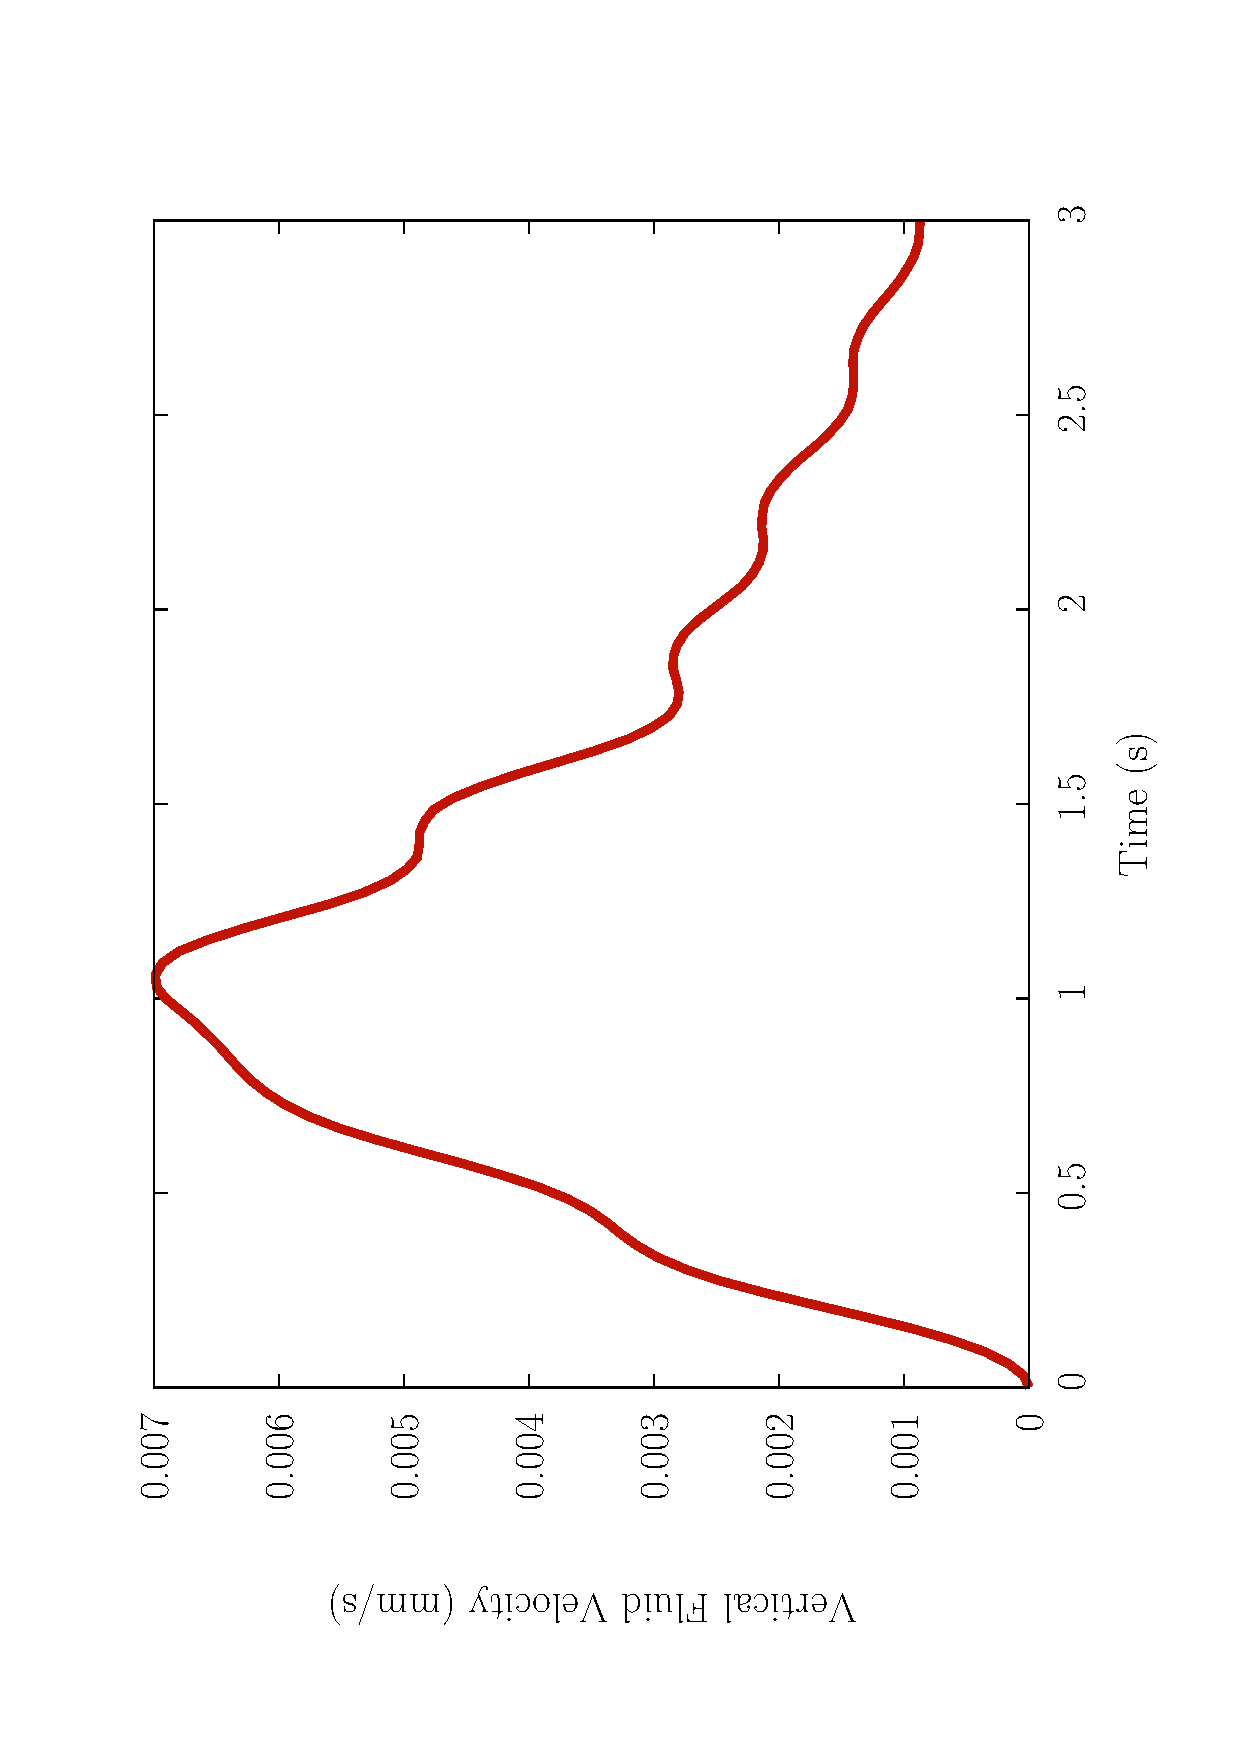
\includegraphics[width=0.6\textwidth,angle=270]{images/examples/eulerian/constriction/constrict-vel-drop-dynamic}
\caption{Vertical fluid velocity evolution with dynamics.} 
\label{velocity-evolution-dynamic}
\end{figure}

\begin{figure}[!hpt]
\centering
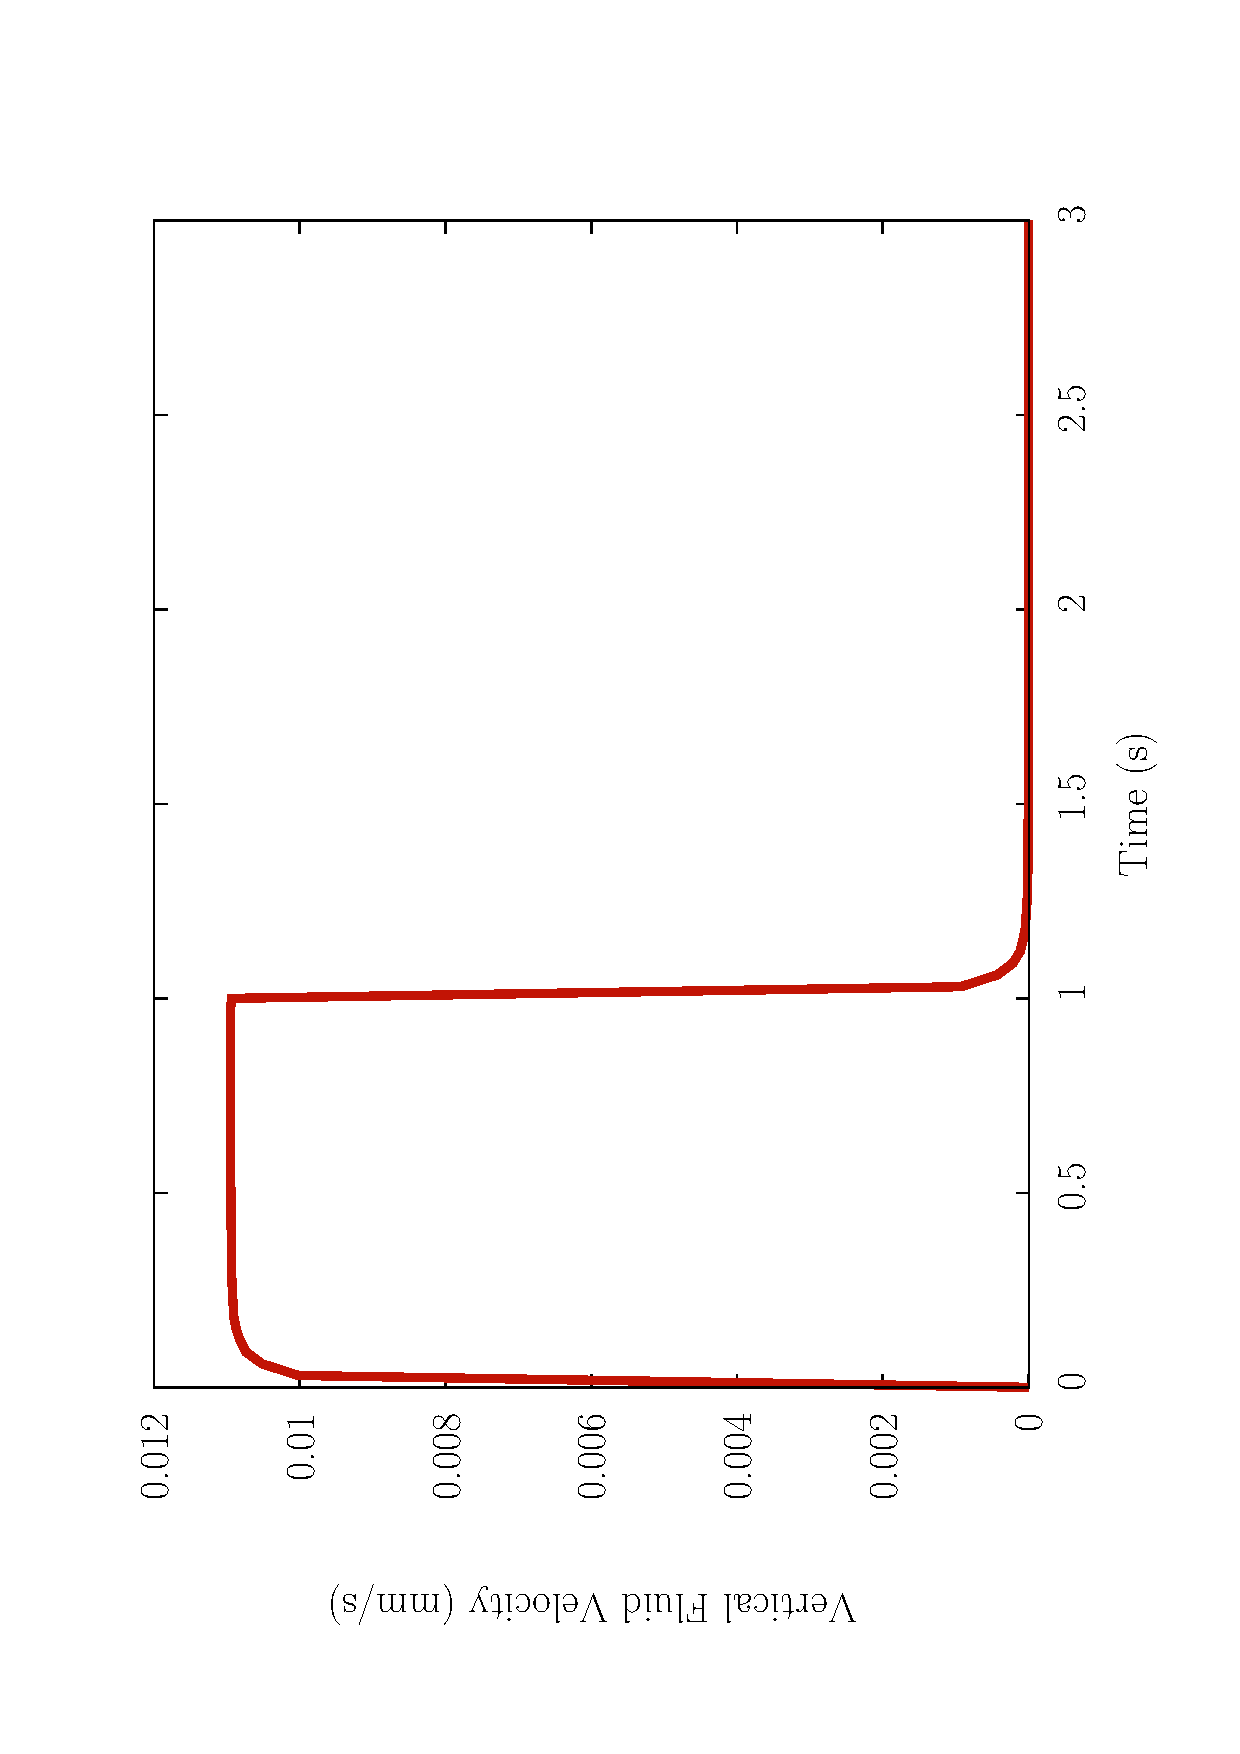
\includegraphics[width=0.6\textwidth,angle=270]{images/examples/eulerian/constriction/constrict-vel-drop-quasistatic}
\caption{Vertical fluid velocity evolution with quasistatics.} 
\label{velocity-evolution-quasistatic}
\end{figure}

\subsection{Flow fields under tension}
\label{tension-flow}

\section{Examples exploring the biphasic nature of porous soft tissue}
\label{biphasic-examples-2}

\subsection{Stress relaxation}
\label{stress-relaxation}
With viscoelasticity and poroelasticity, quasistatic and dynamic.

\subsection{Hysteresis}
\label{hysteresis}
With viscoelasticity and poroelasticity, quasistatic and dynamic.

\section{Tumour growth}
\label{tumour-growth}

\subsection{Isotropic swelling}
\label{tumour-isotropic-swelling}

\begin{figure}[!hpt]
\centering
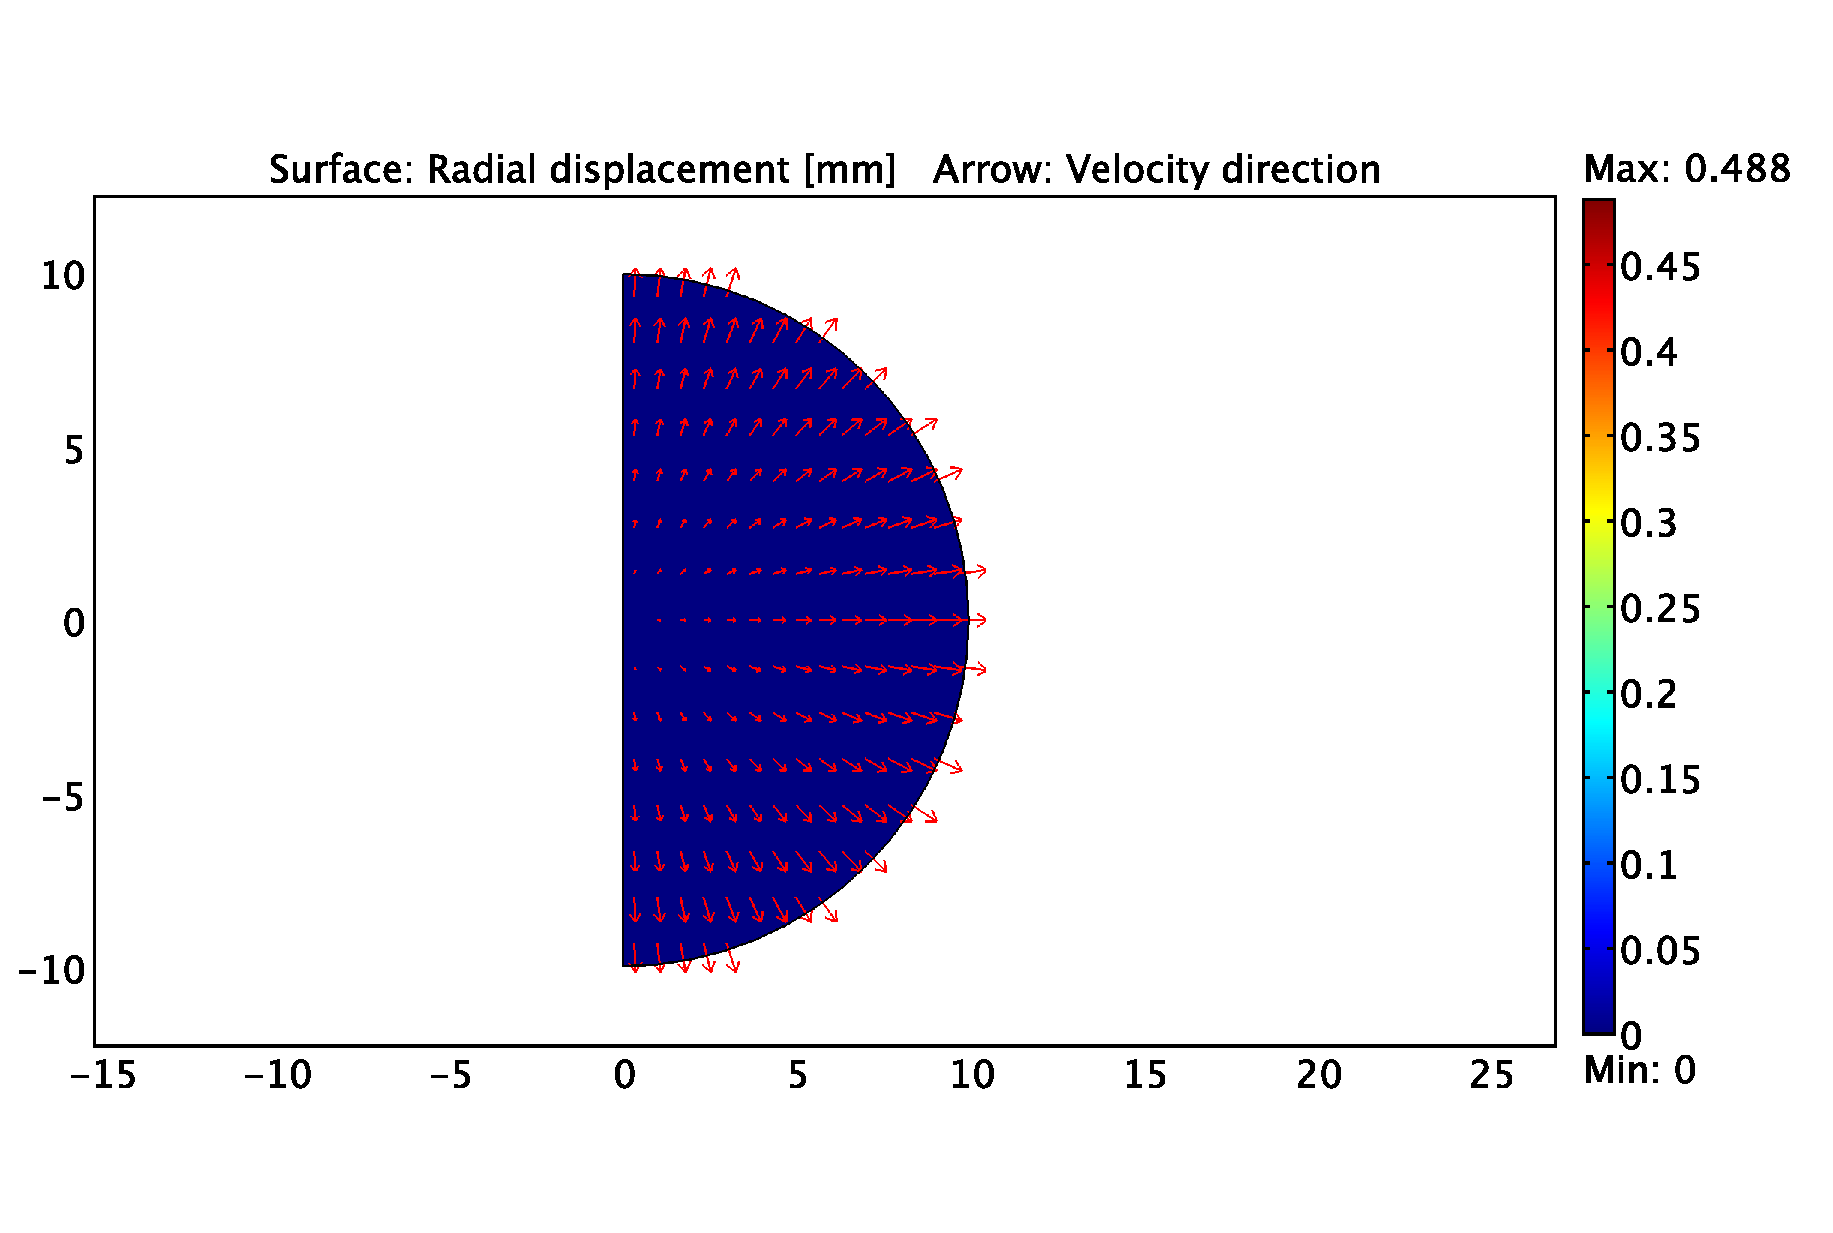
\includegraphics[width=0.8\textwidth]{images/examples/eulerian/cancer/isotropic-swelling-0}
\caption{A semicircular tumour at time $t=0$ days.}
\label{tumour-isotropic-swelling-0}
\end{figure}

\begin{figure}[!hpt]
\centering
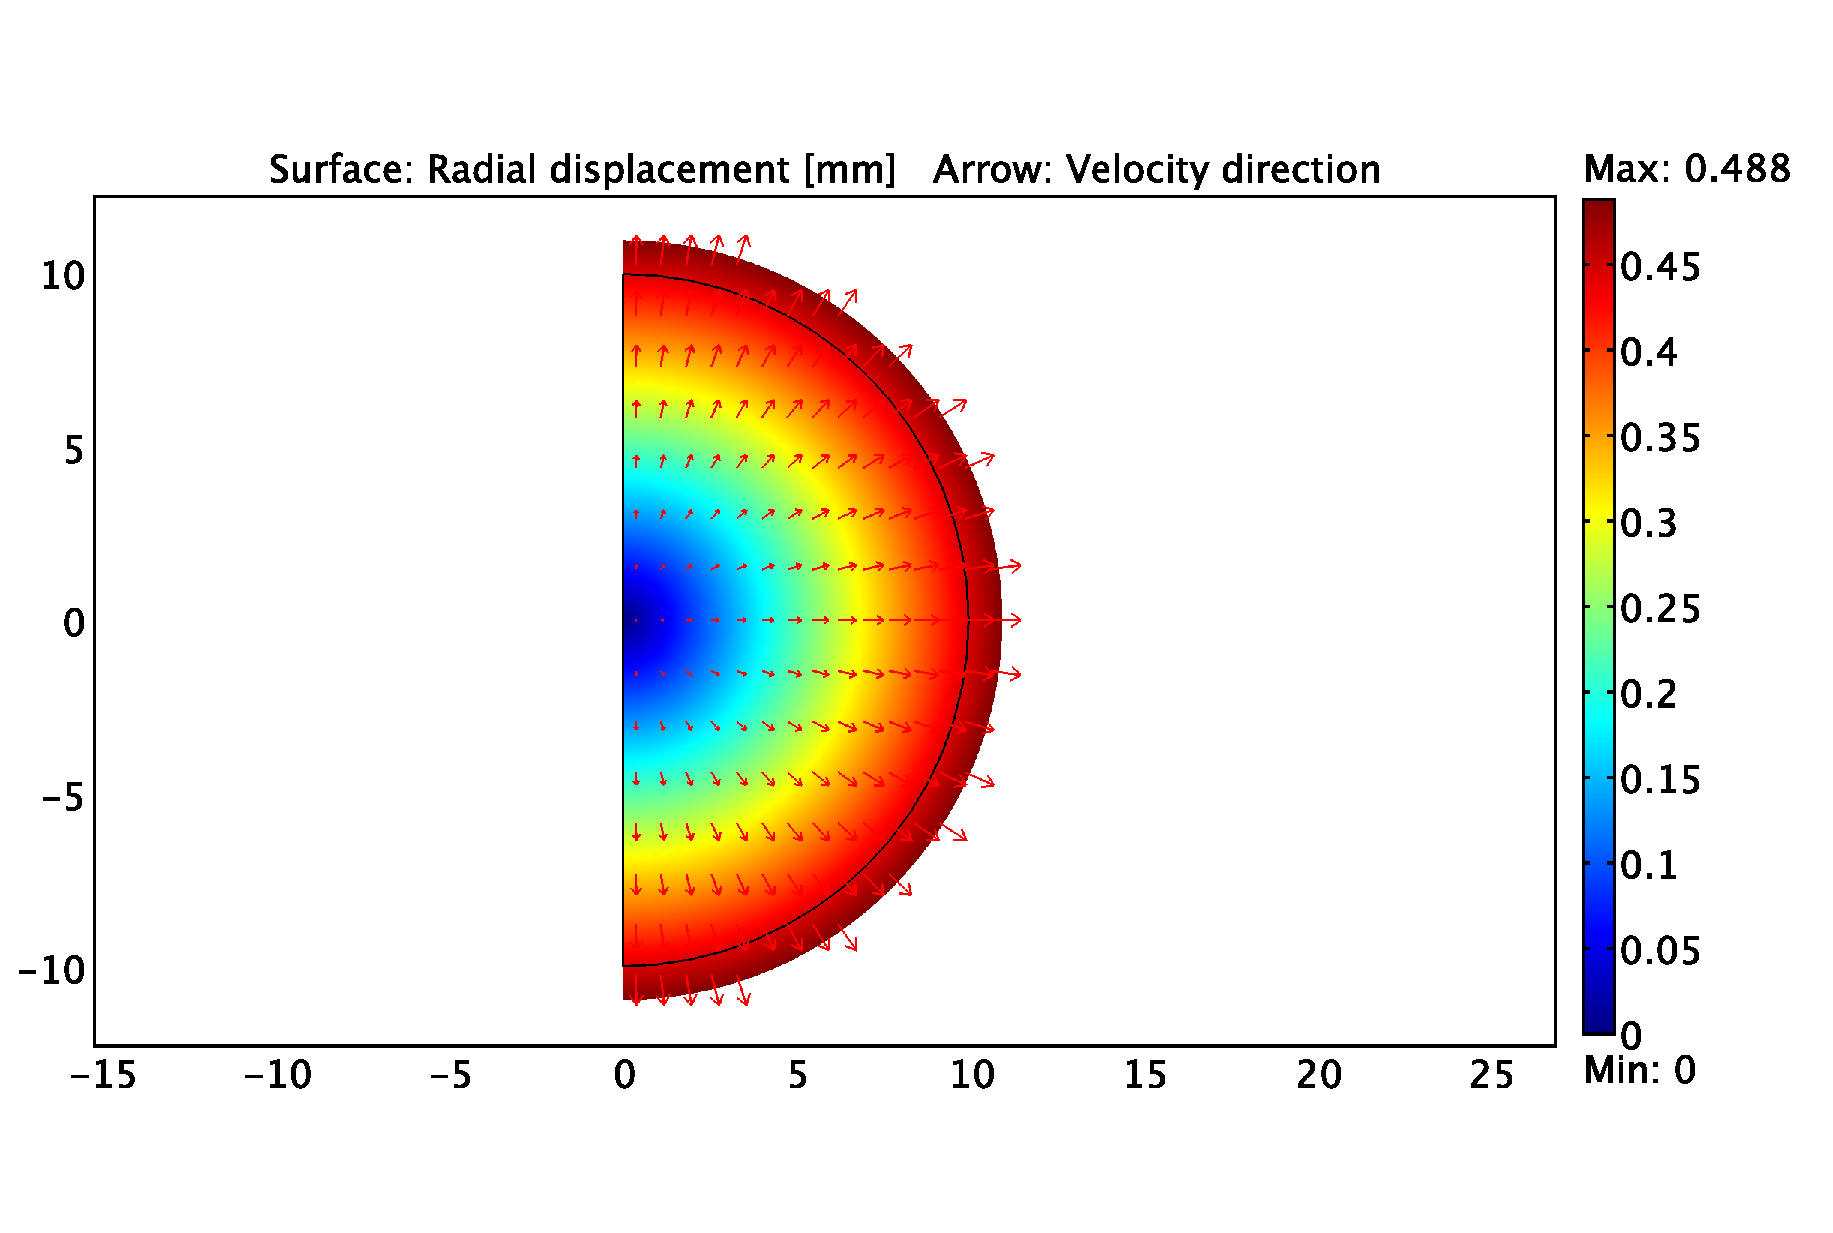
\includegraphics[width=0.8\textwidth]{images/examples/eulerian/cancer/isotropic-swelling-100}
\caption{A semicircular tumour at time $t=100$ days.}
\label{tumour-isotropic-swelling-100}
\end{figure}

\begin{figure}[!hpt]
\centering
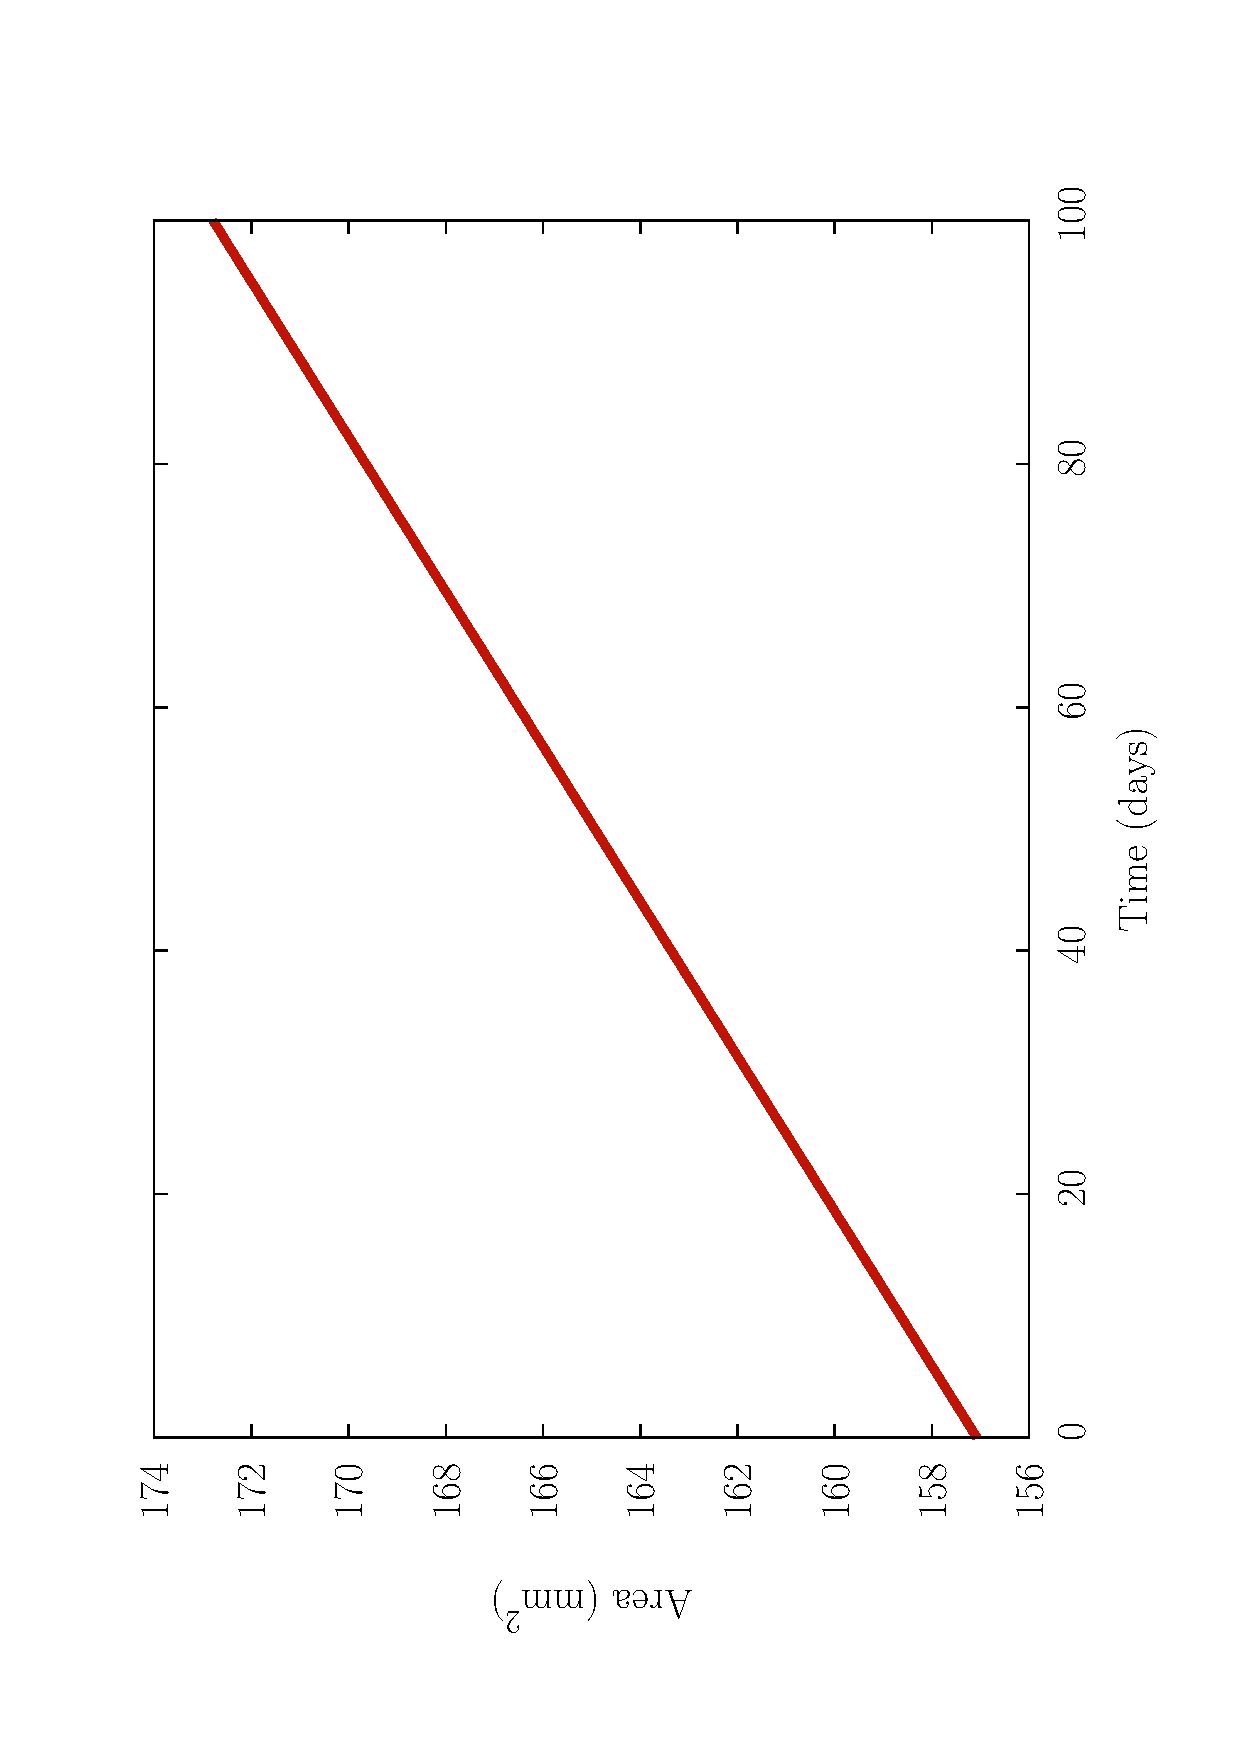
\includegraphics[width=0.6\textwidth,angle=270]{images/examples/eulerian/cancer/isotropic-swelling-area-evolution}
\caption{The area of the tumour evolving over 100 days.}
\label{tumour-isotropic-area-evolution}
\end{figure}

\subsection{Constrained by a wall}
\label{wall-constraint}

\begin{figure}[!hpt]
\centering
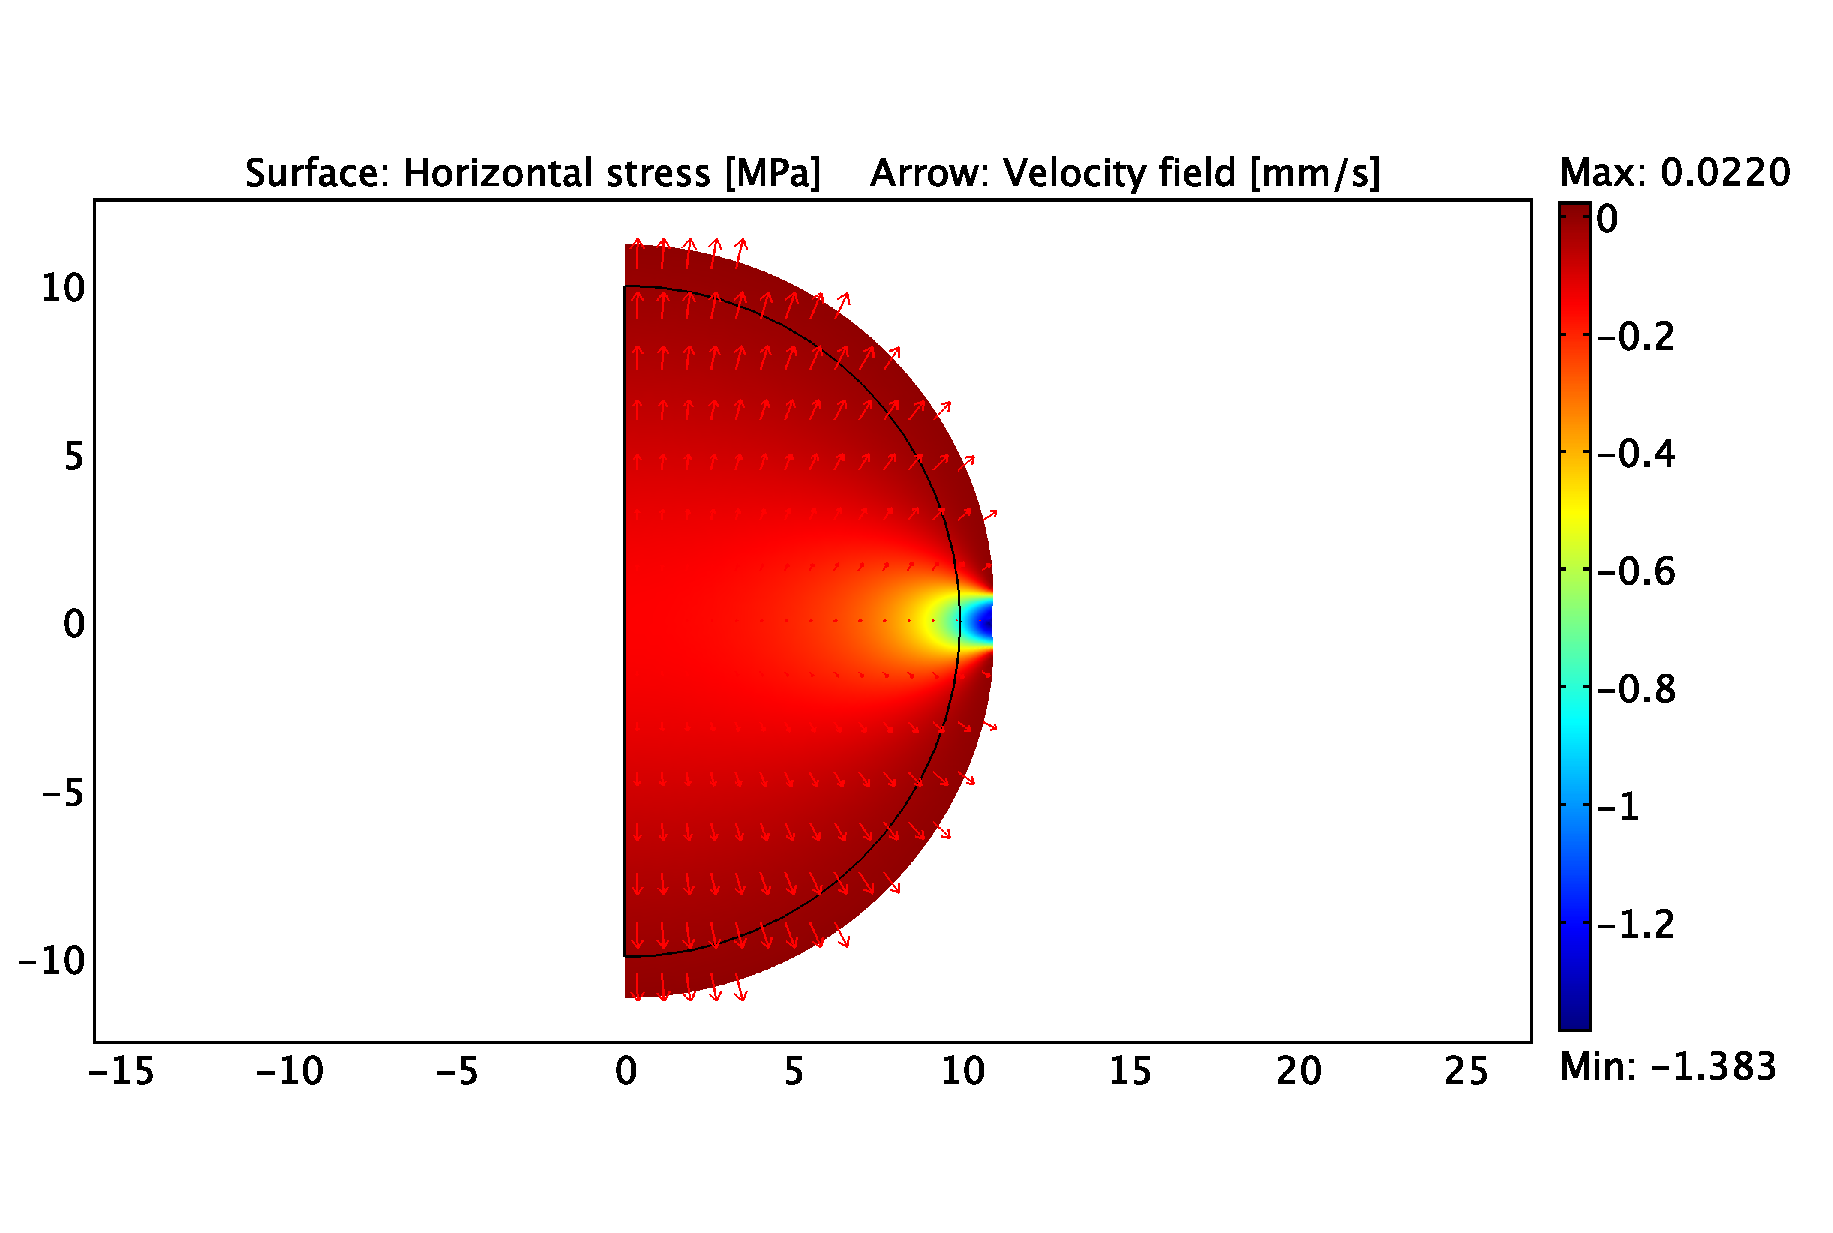
\includegraphics[width=0.8\textwidth]{images/examples/eulerian/cancer/constrained-swelling-120}
\caption{The growing tumour constrained by a wall at time $t=100$ days.}
\label{tumour-constrained-swelling-120}
\end{figure}

\begin{figure}[!hpt]
\centering
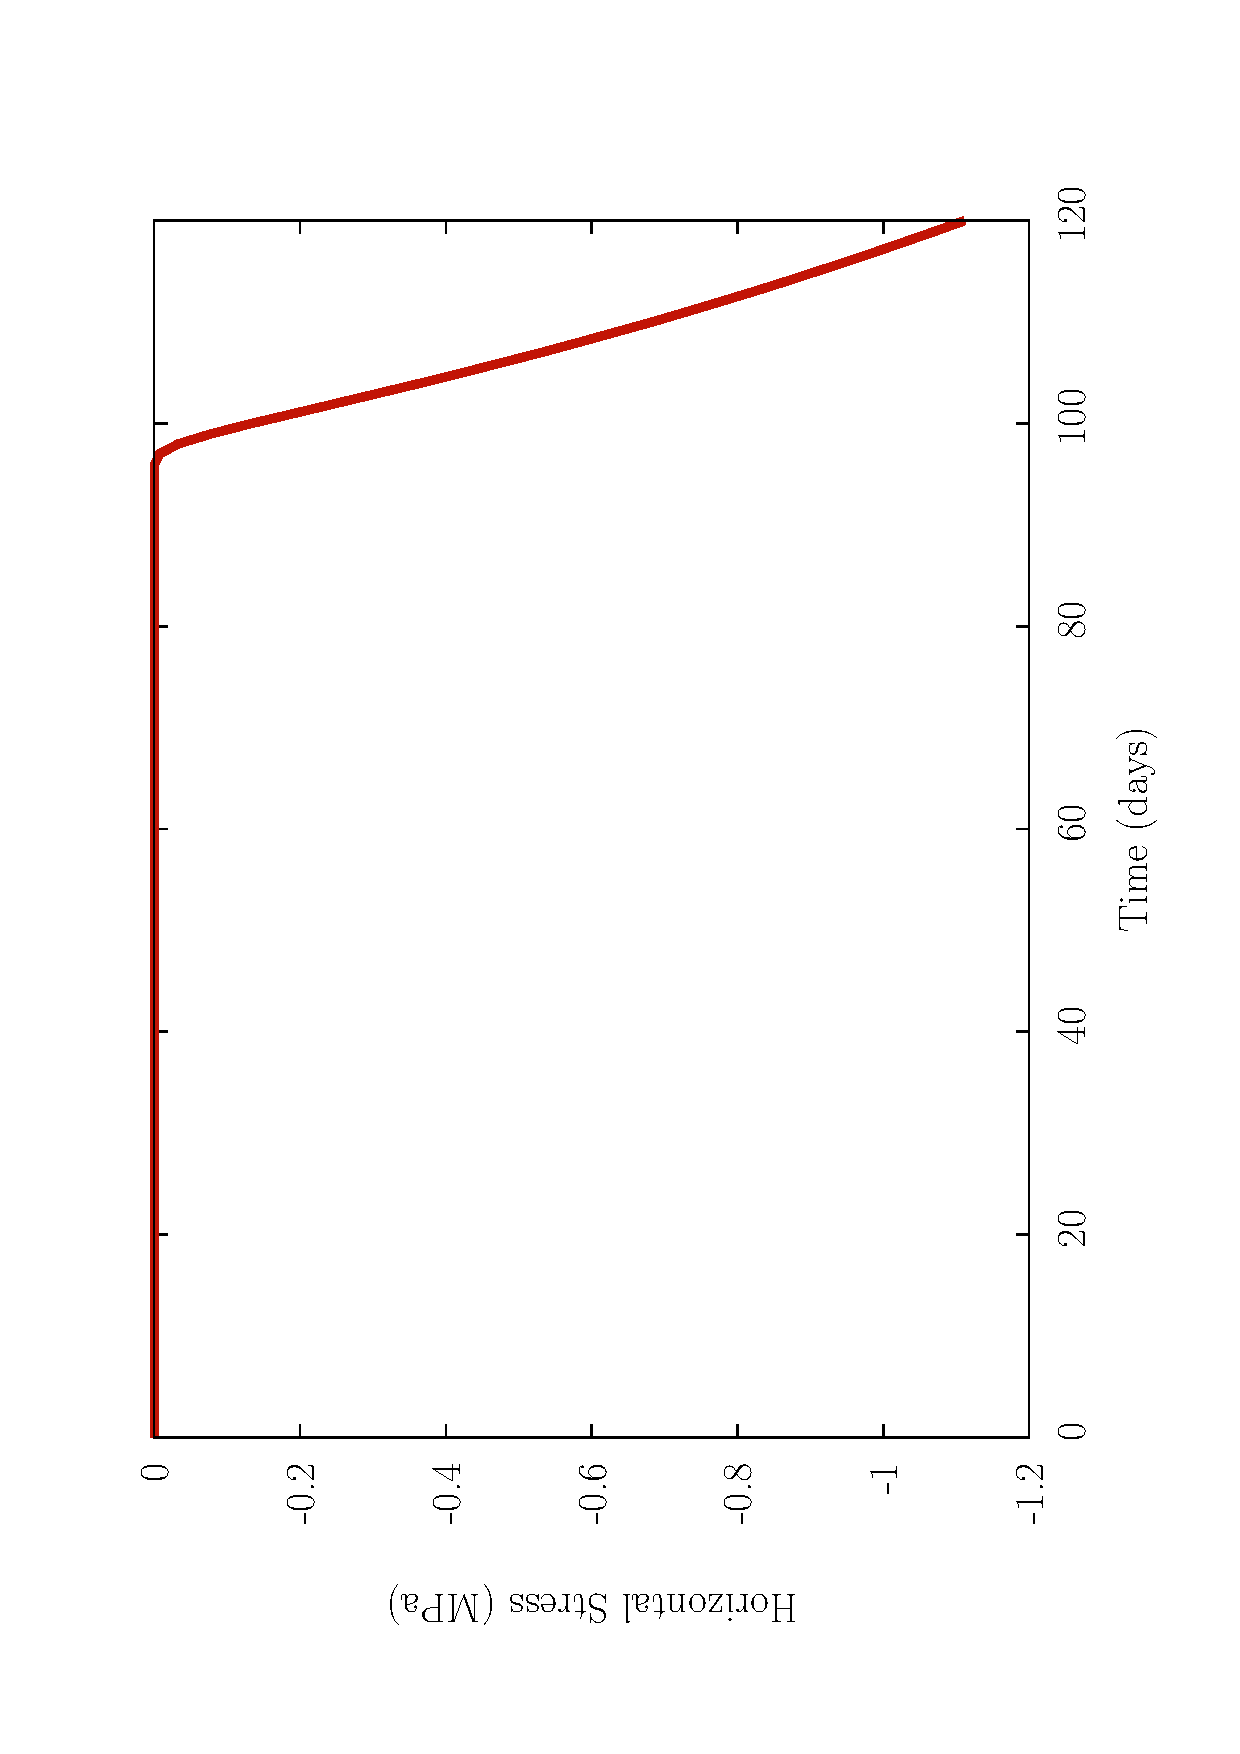
\includegraphics[width=0.6\textwidth,angle=270]{images/examples/eulerian/cancer/constrained-stress-evolution}
\caption{The horizontal stress in the tumour evolving over 120 days.}
\label{tumour-constrained-stress-evolution}
\end{figure}

\subsection{The role of the cells}
\label{cell-roles}

\subsubsection{Inward tug}
\label{inward-tug}

\begin{figure}[!hpt]
\centering
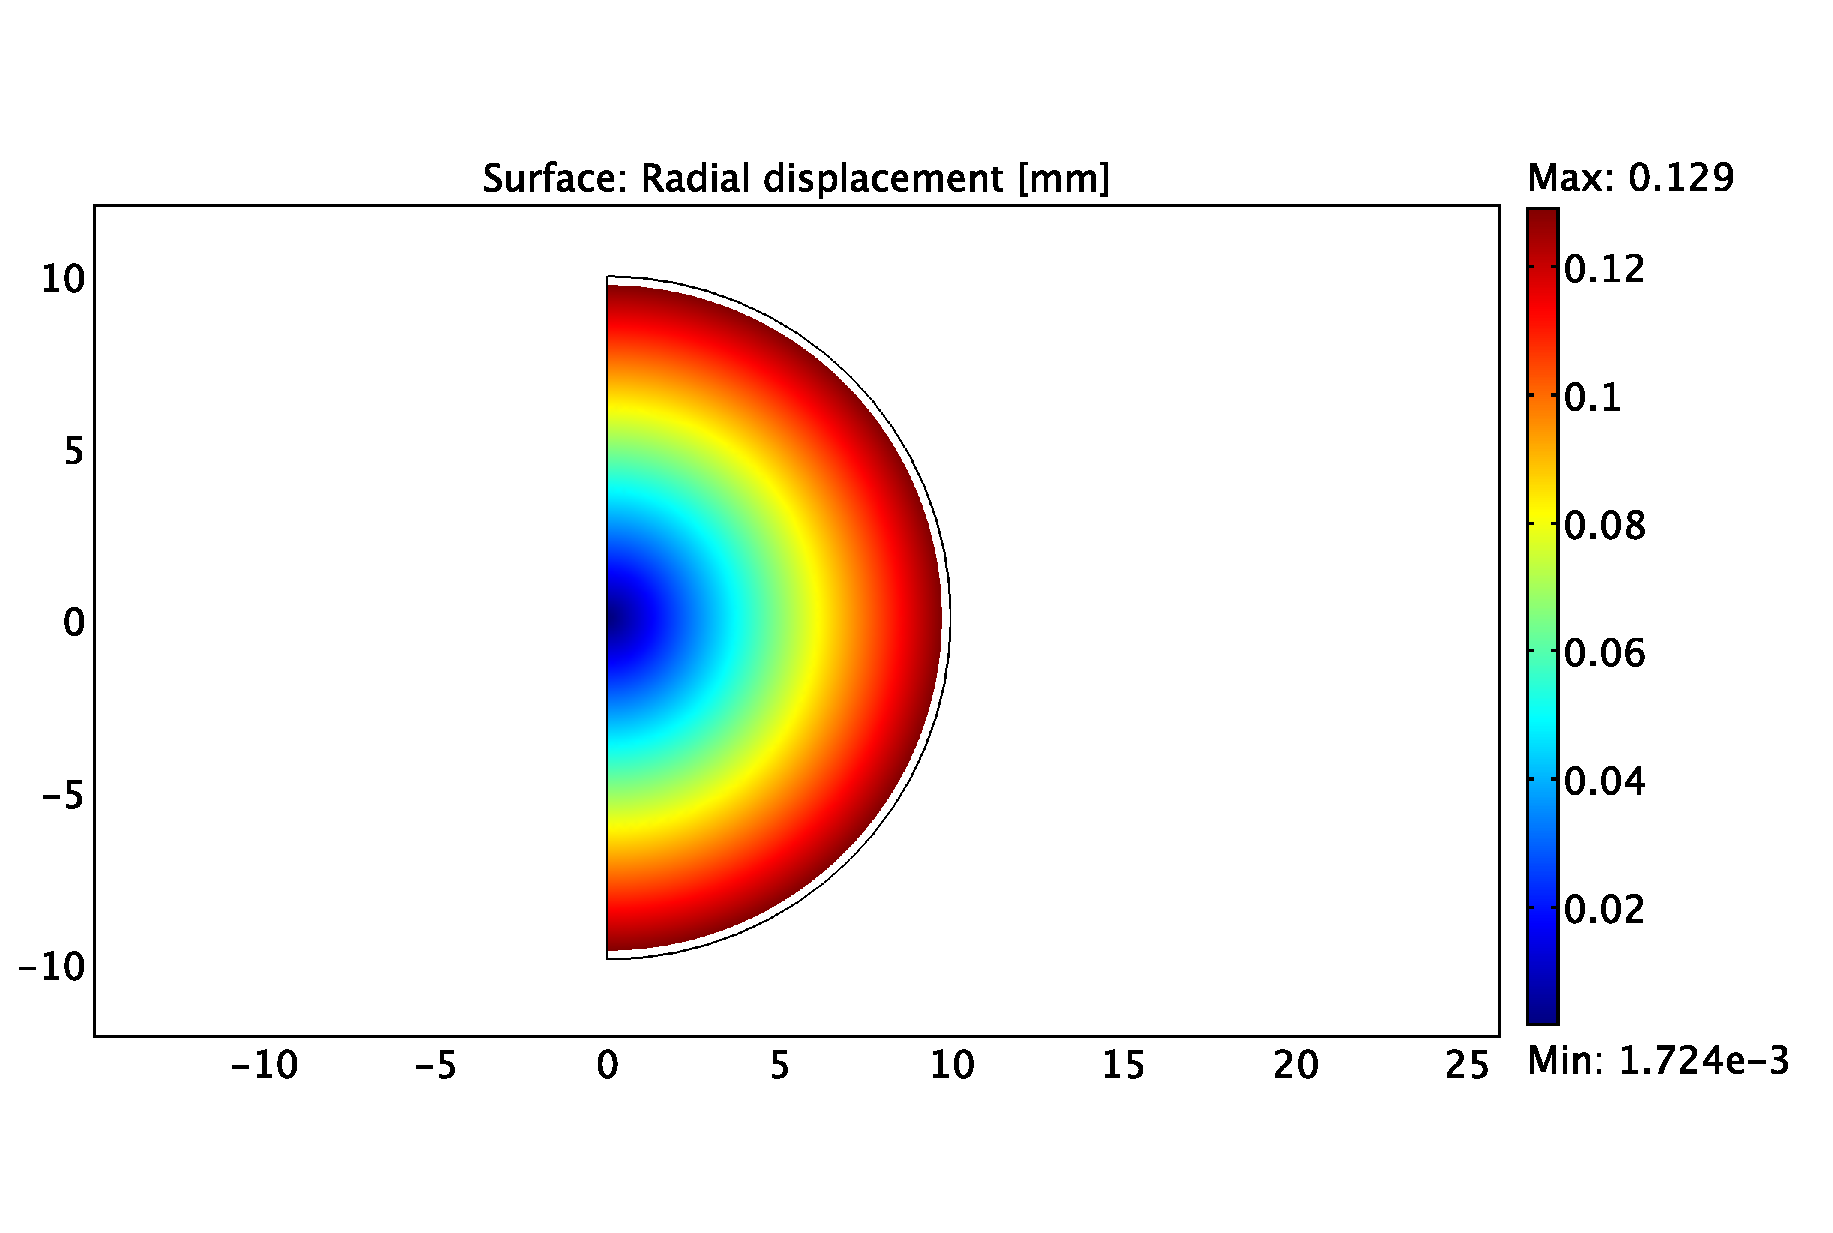
\includegraphics[width=0.8\textwidth]{images/examples/eulerian/cancer/homogeneous-inward-tug}
\caption{Homogeneous inward tug due to a uniform distribution of cells.}
\label{tumour-homogeneous-inward-tug}
\end{figure}

\begin{figure}[!hpt]
\centering
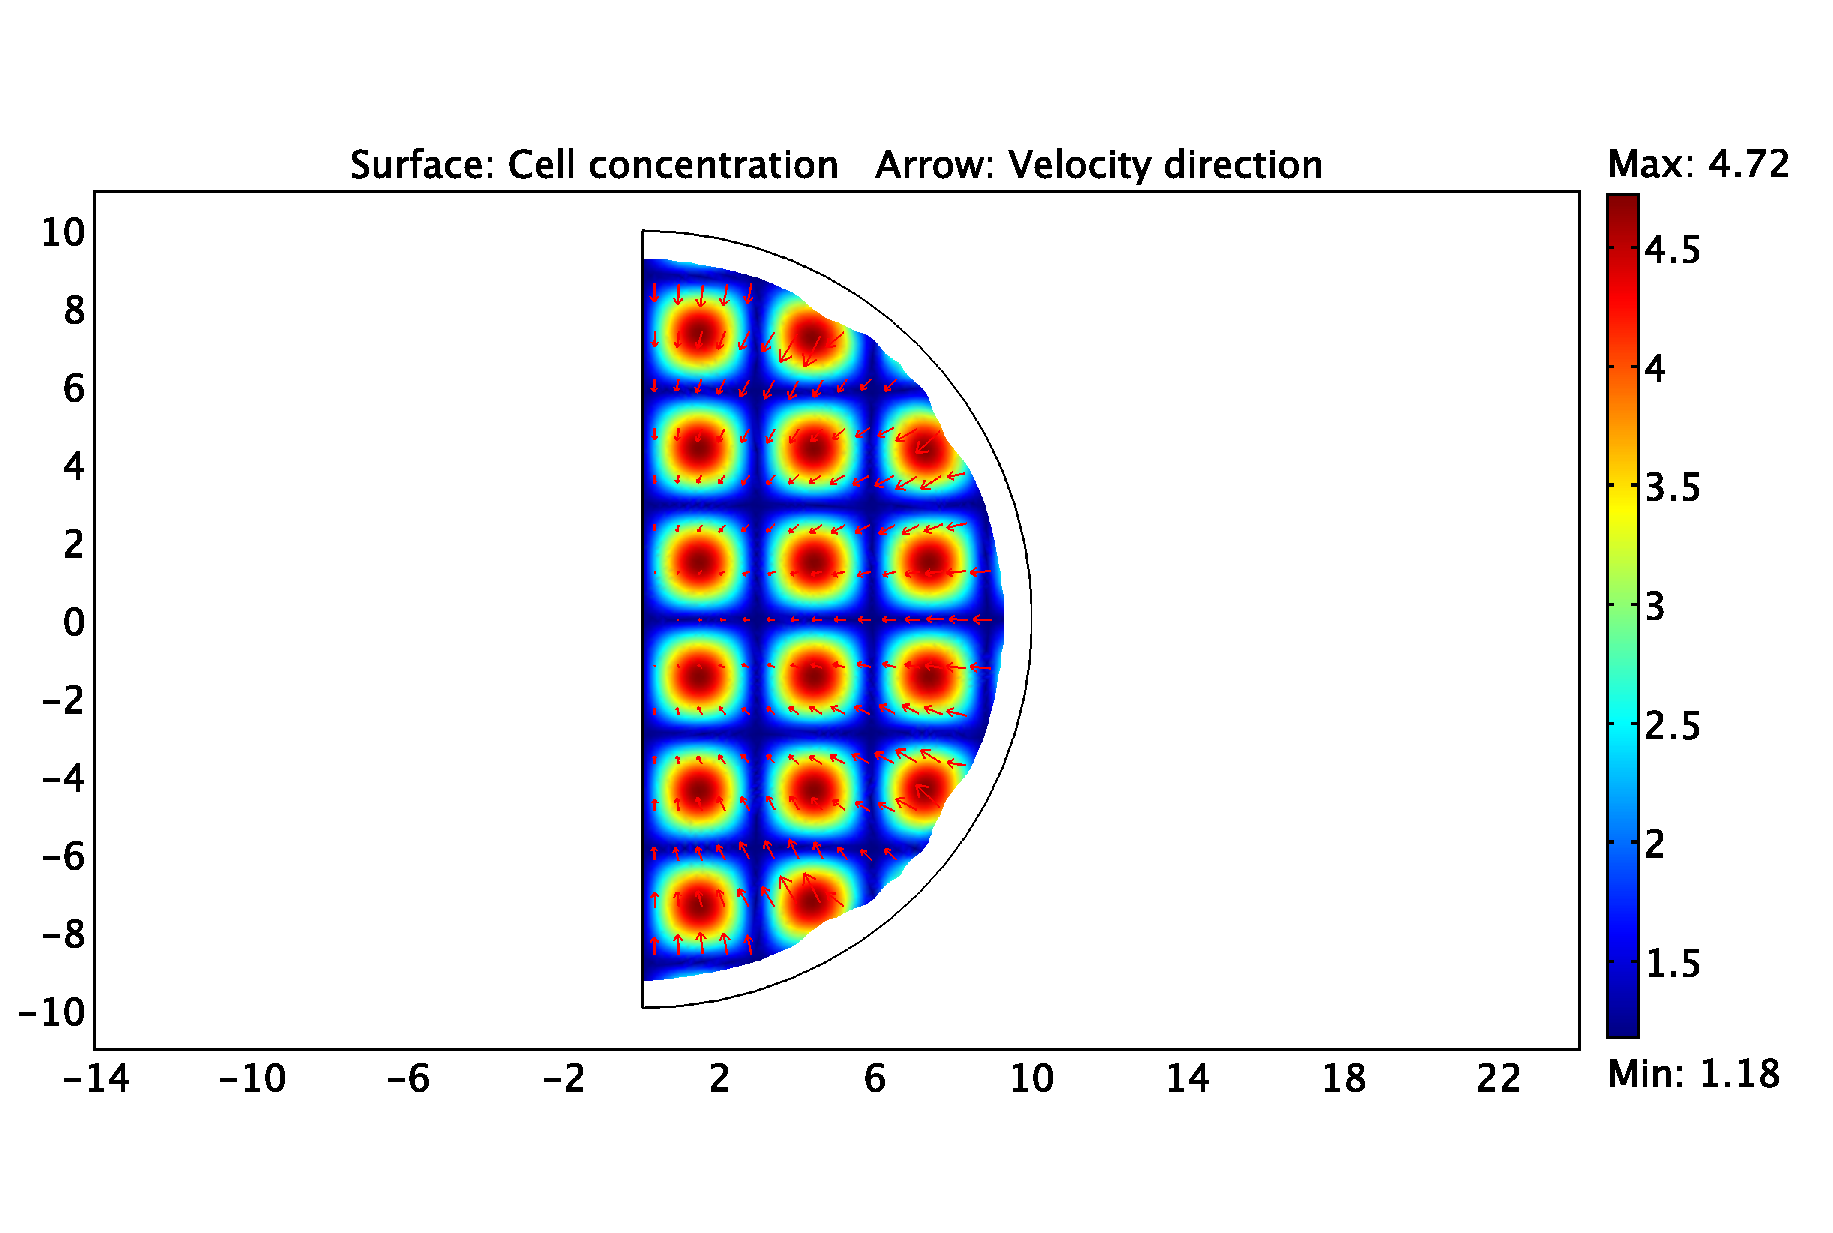
\includegraphics[width=0.8\textwidth]{images/examples/eulerian/cancer/heterogeneous-inward-tug}
\caption{Heterogeneous inward tug due to a non-uniform distribution of cells.}
\label{tumour-heterogeneous-inward-tug}
\end{figure}

\subsubsection{Transport of the cells}
\label{cell-transport}

\begin{figure}[!hpt]
\centering
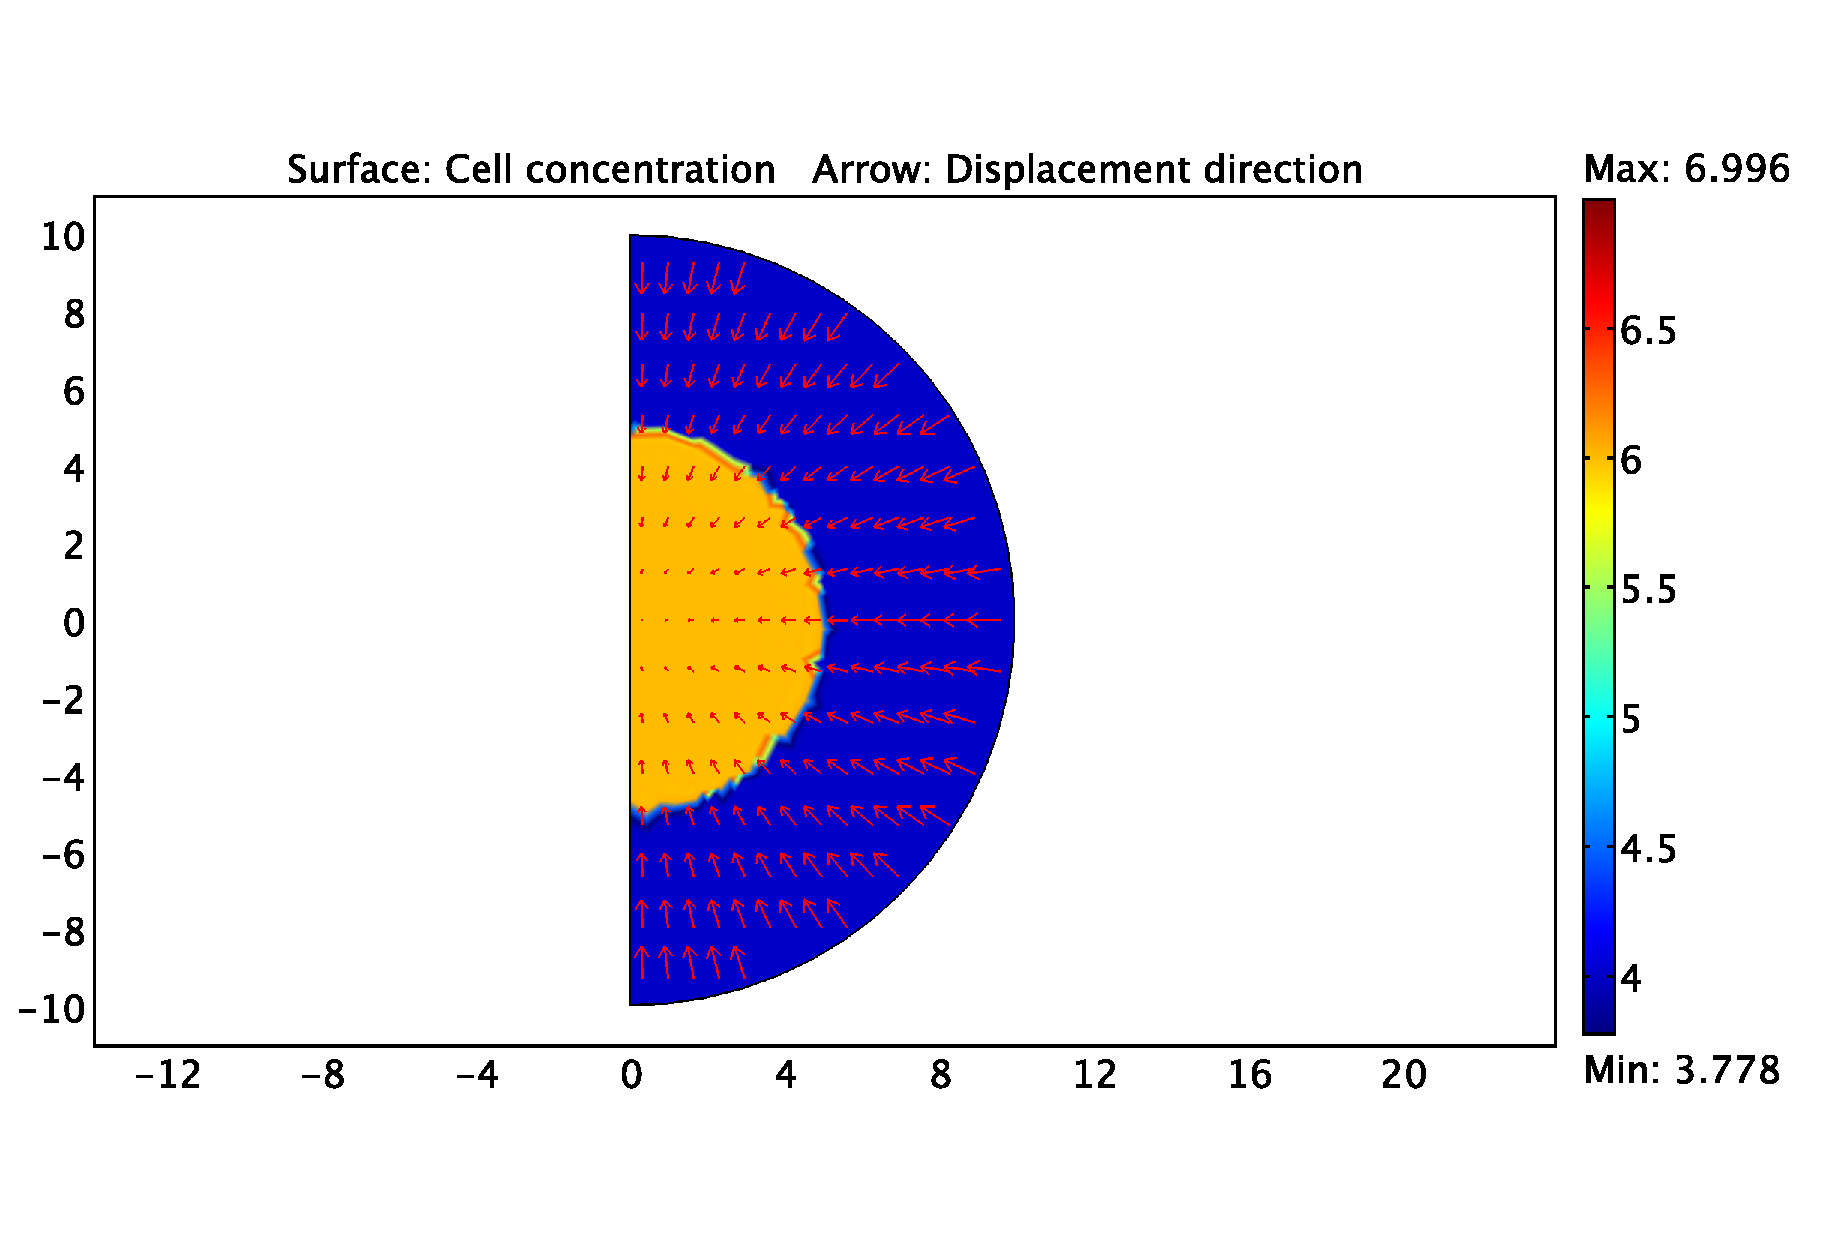
\includegraphics[width=0.8\textwidth]{images/examples/eulerian/cancer/diffusing-proliferating-cells-0}
\caption{The cells diffusing and proliferating at time $t=0$ days.}
\label{tumour-diffusion-proliferation-0}
\end{figure}

\begin{figure}[!hpt]
\centering
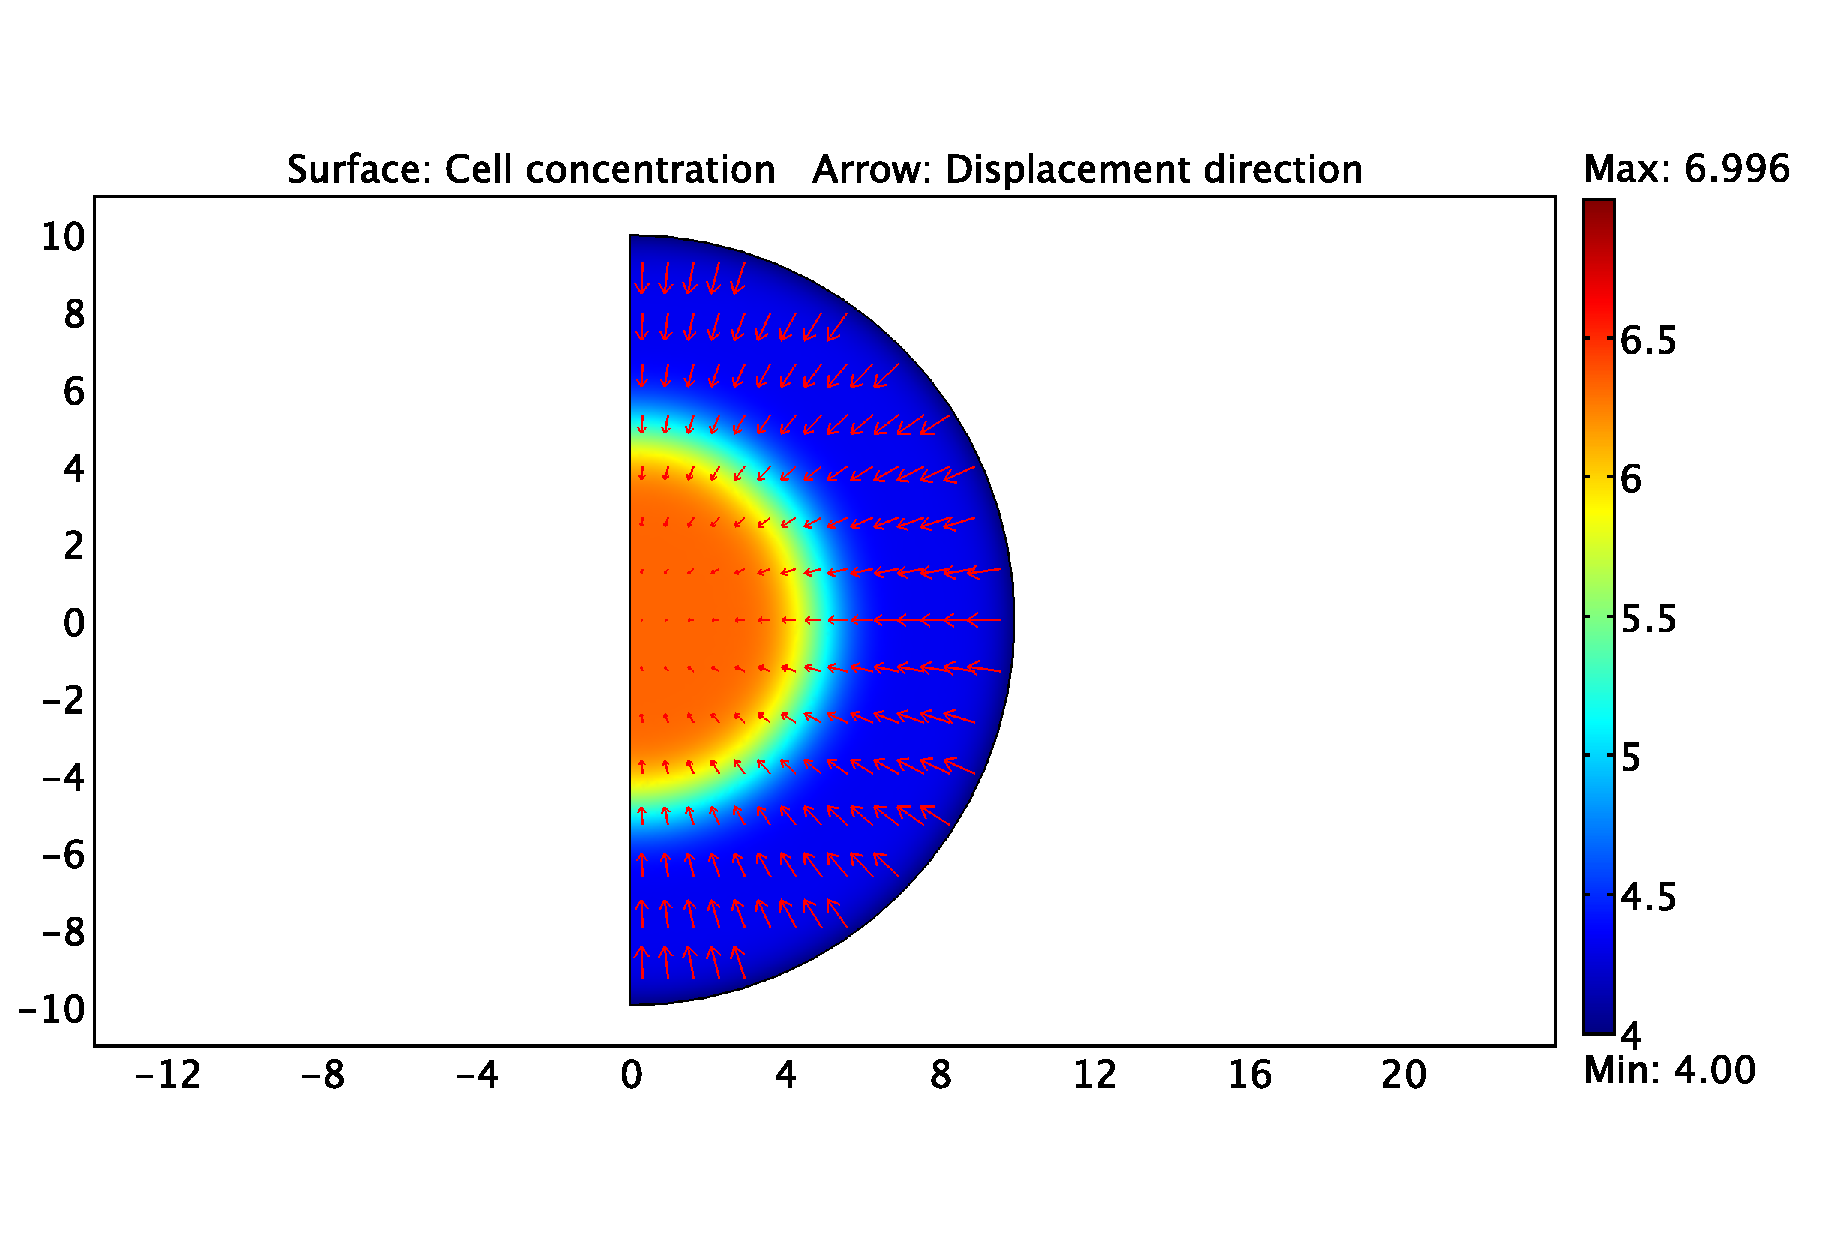
\includegraphics[width=0.8\textwidth]{images/examples/eulerian/cancer/diffusing-proliferating-cells-33}
\caption{The cells diffusing and proliferating at time $t=33$ days.}
\label{tumour-diffusion-proliferation-33}
\end{figure}

\begin{figure}[!hpt]
\centering
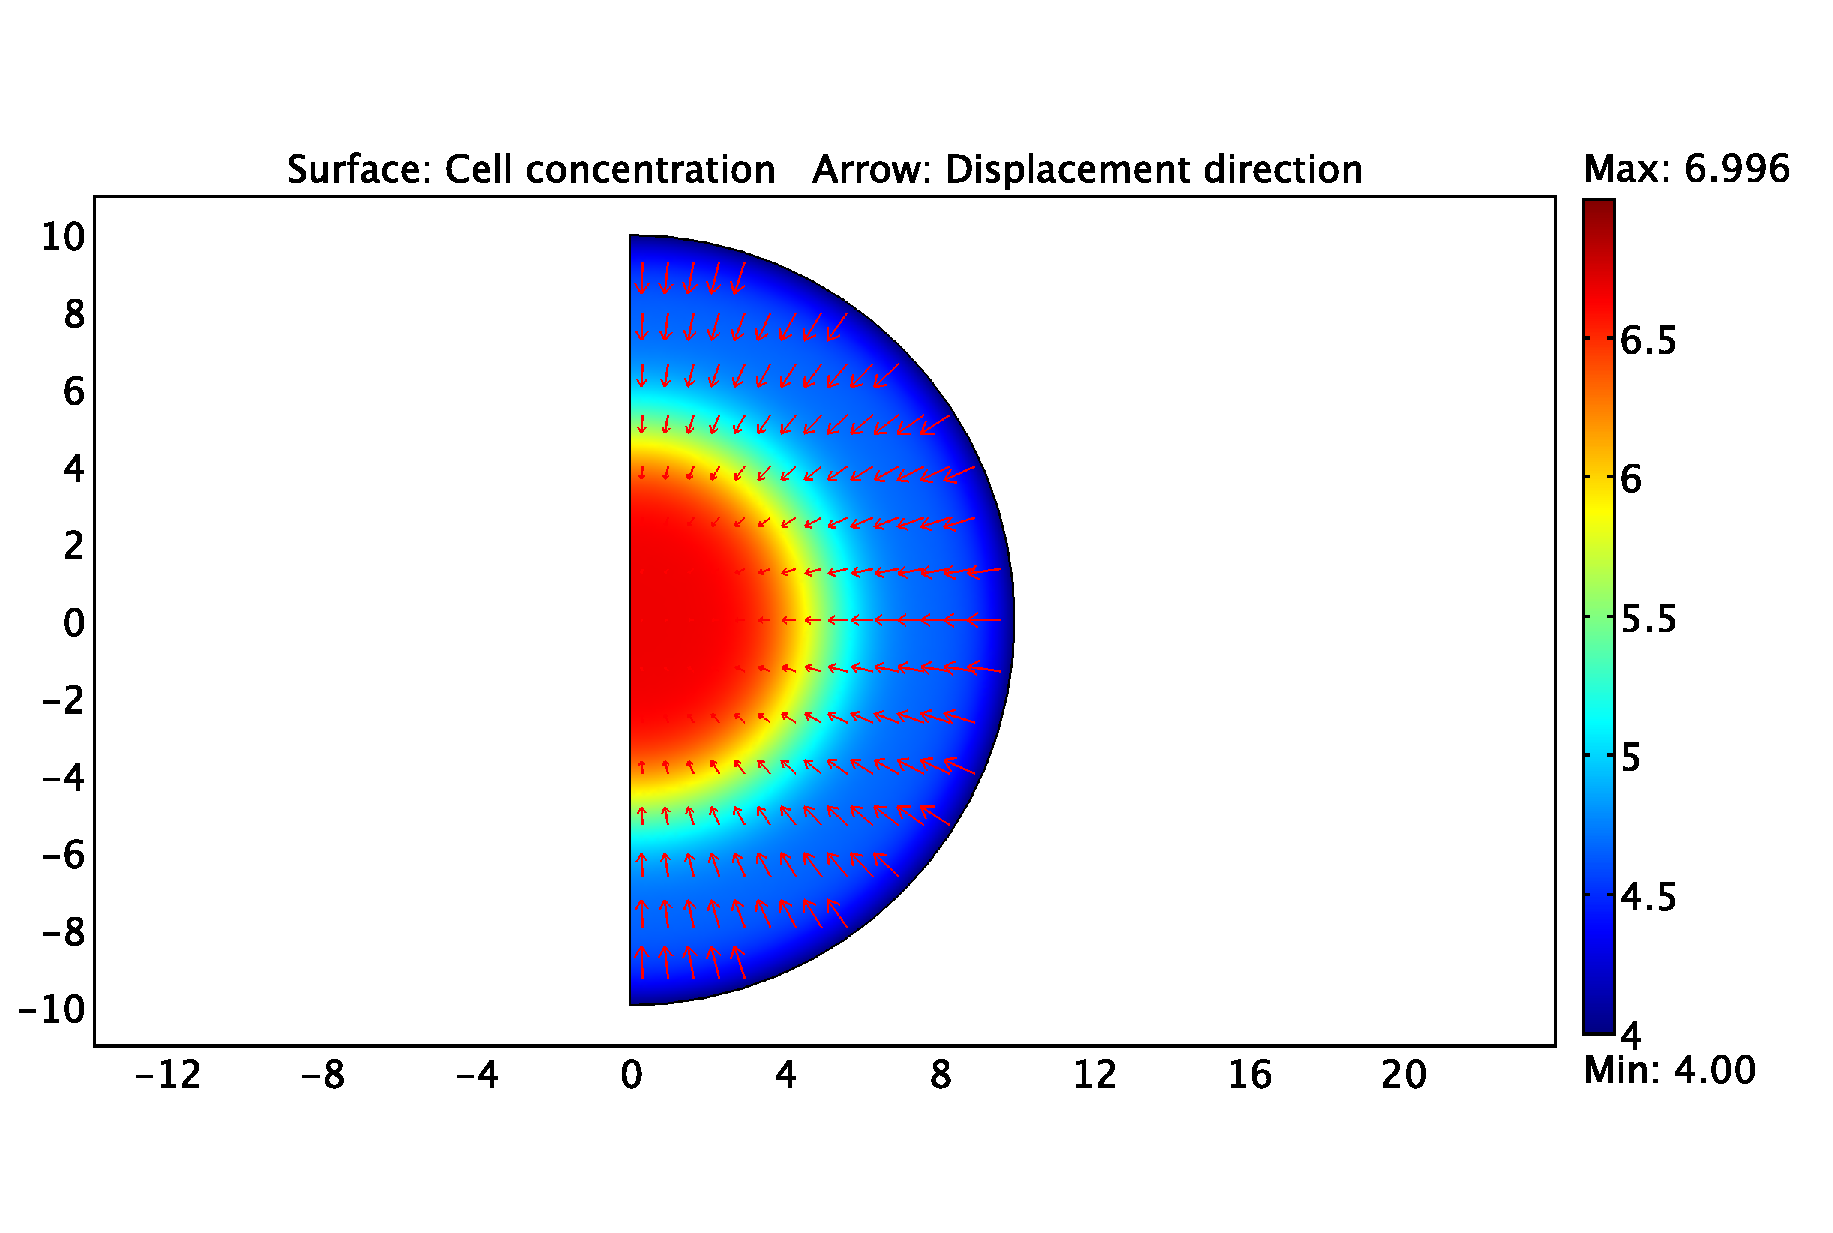
\includegraphics[width=0.8\textwidth]{images/examples/eulerian/cancer/diffusing-proliferating-cells-67}
\caption{The cells diffusing and proliferating at time $t=67$ days.}
\label{tumour-diffusion-proliferation-67}
\end{figure}

\begin{figure}[!hpt]
\centering
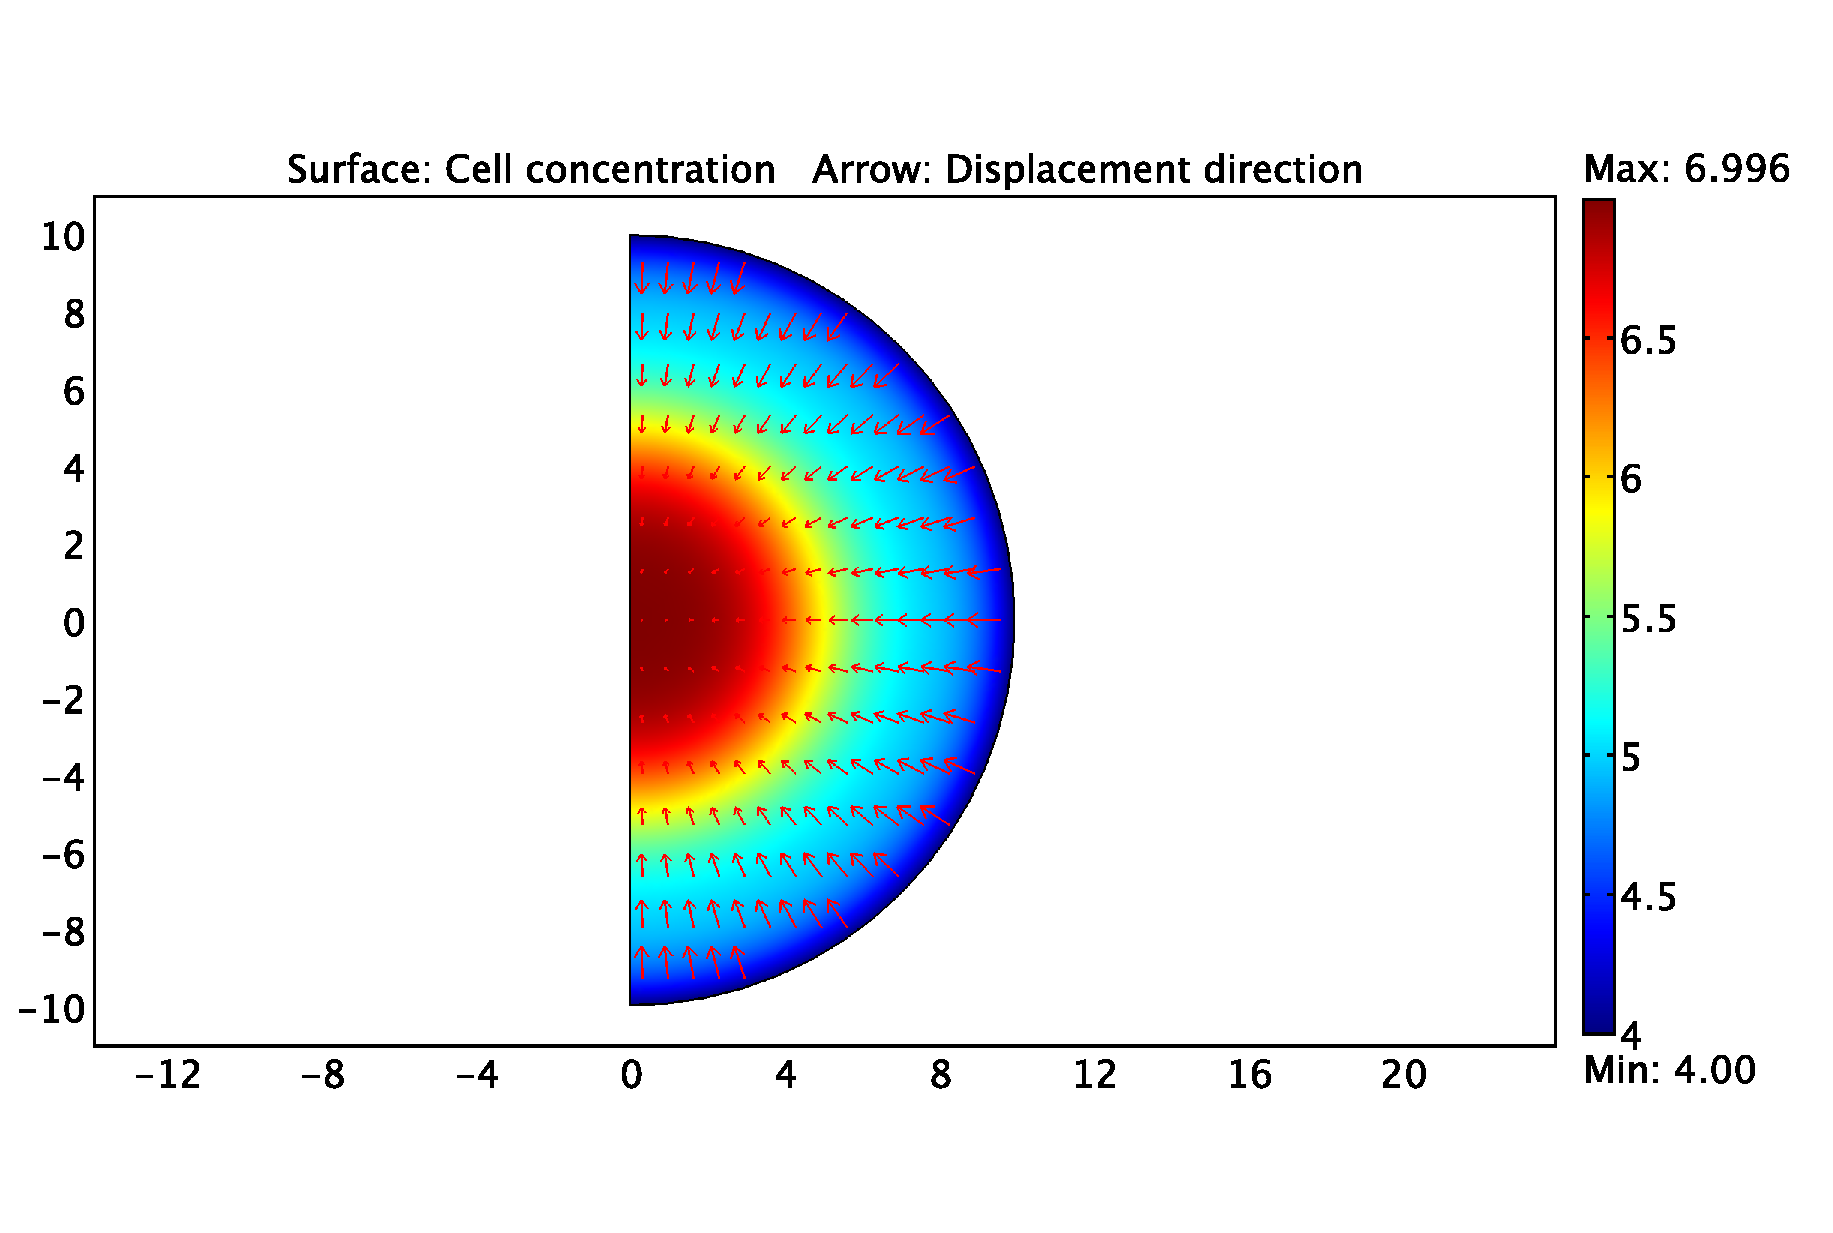
\includegraphics[width=0.8\textwidth]{images/examples/eulerian/cancer/diffusing-proliferating-cells-100}
\caption{The cells diffusing and proliferating at time $t=100$ days.}
\label{tumour-diffusion-proliferation-100}
\end{figure}


%

% Local Variables:
% TeX-master: "thesis"
% mode: latex
% mode: flyspell
% End:
